\documentclass[]{article}
\usepackage{graphicx}
\usepackage{hyperref}
\usepackage{amsmath}
\usepackage{caption}
\usepackage{subcaption}
\usepackage{float}


%opening
\title{VME Data Acquisition and Plastic Scintillators}
\author{Gunther T\"urk, Jonas Lehnen}

\begin{document}

\maketitle
\begin{abstract}


\end{abstract}

\tableofcontents

\newpage
\section{Theorie}
Questions 

Please answer the following questions shortly (Do not exceed one page of A4 paper to answer them). 
What is isomeric transition (IT)? 
There is a nucleus with Z (atomic number) and A (atomic weight). During the isomeric transition, how can Z and A be changed? 
What is an internal conversion (conversion electron) and what is $\gamma$-decay? 
Explain the difference between $\beta ^-$-decay and the internal conversion? 

Problems 

The following problems are specified questions for this experiment. Please answer them as well. 


Problem 1 






Picture 2.1: Electron Capture Decay Scheme




Picture 2.2: Isomeric Transition Decay Scheme 

${}^{207}Bi$ was first reported by Neumann and Perlman. Consult the references about the more information about ${}^{207}Bi$: 
Internal Conversion and Directional Angular Correlation of the Bi207 Gammas - F. K. McGowan and E. C. Campbell 
Internal Conversion Electron-Gamma Directional Angular Correlation of Bi207 - F. K. McGowan  
The Isomeric Transition of Pb207 as an Energy Standard in Beta Spectroscopy - David E. Alburger 
Decay of Bi207 - N. H. Lazar and E. D. Klema  
(L+M+. . .)/K capture ratio in the decay of 207Bi - A M Mandal and A P Patro 


Explain the following decay schema individually and what is the difference between the two decay schema (Fig. 2.1 and Fig. 2.2)? 


Problem 2 

Atomic-electron binding energies of ${}^{82}$ is the following (see book Modern atomic and nuclear physics F Yang, JH Hamilton - 1996 ) 








Problem 3 

Which are the three major processes of an interaction mechanismn for $\gamma$-rays in matter? Explain theses processes in more detail. 

Problem 4 

Photons with 3 MeV energy are counted by a NaI(TI) detector. Sketch the expected spectrum and explain what you sketch and the physics process beneath it. 

Problem 5 

Explain how a plastic scintillation counter works, from the incoming of a charged particle or $\gamma$ in a plastic scintillator to the output signal of the PMT. 

Problem 6 

How many counts are needed to make the standard deviation equal to 1%? And if one obtains 8423456 counts in 300 seconds, what is the standard deviation of the count rate? 

\subsection{Radiation}\label{radiation}
%%% describe 207 Bismuth - decay modes

\subsection{Scintillator}\label{scintillator}
A scintillator is a material that exhibits light, when excited by ionizing radiation. In our experiment we use a two meter plastic scintillator with a photomultiplier at each end to detect the decay of a Bismuth source and background radiation.
\subsection{Refraction index}\label{refrac index}


\newpage
\section{Experiment}
\subsection{Setup}\label{setup}
This experiment we are using a long and flat plastic scintillator to detect high energetic photons or charged particles like cosmic muons. The scintillator is connected with two photo multipliers (PMT) on each side, see figure \ref{fig:setup}.

\begin{figure}[H]
\centering
\begin{subfigure}[h]{0.4\textwidth}
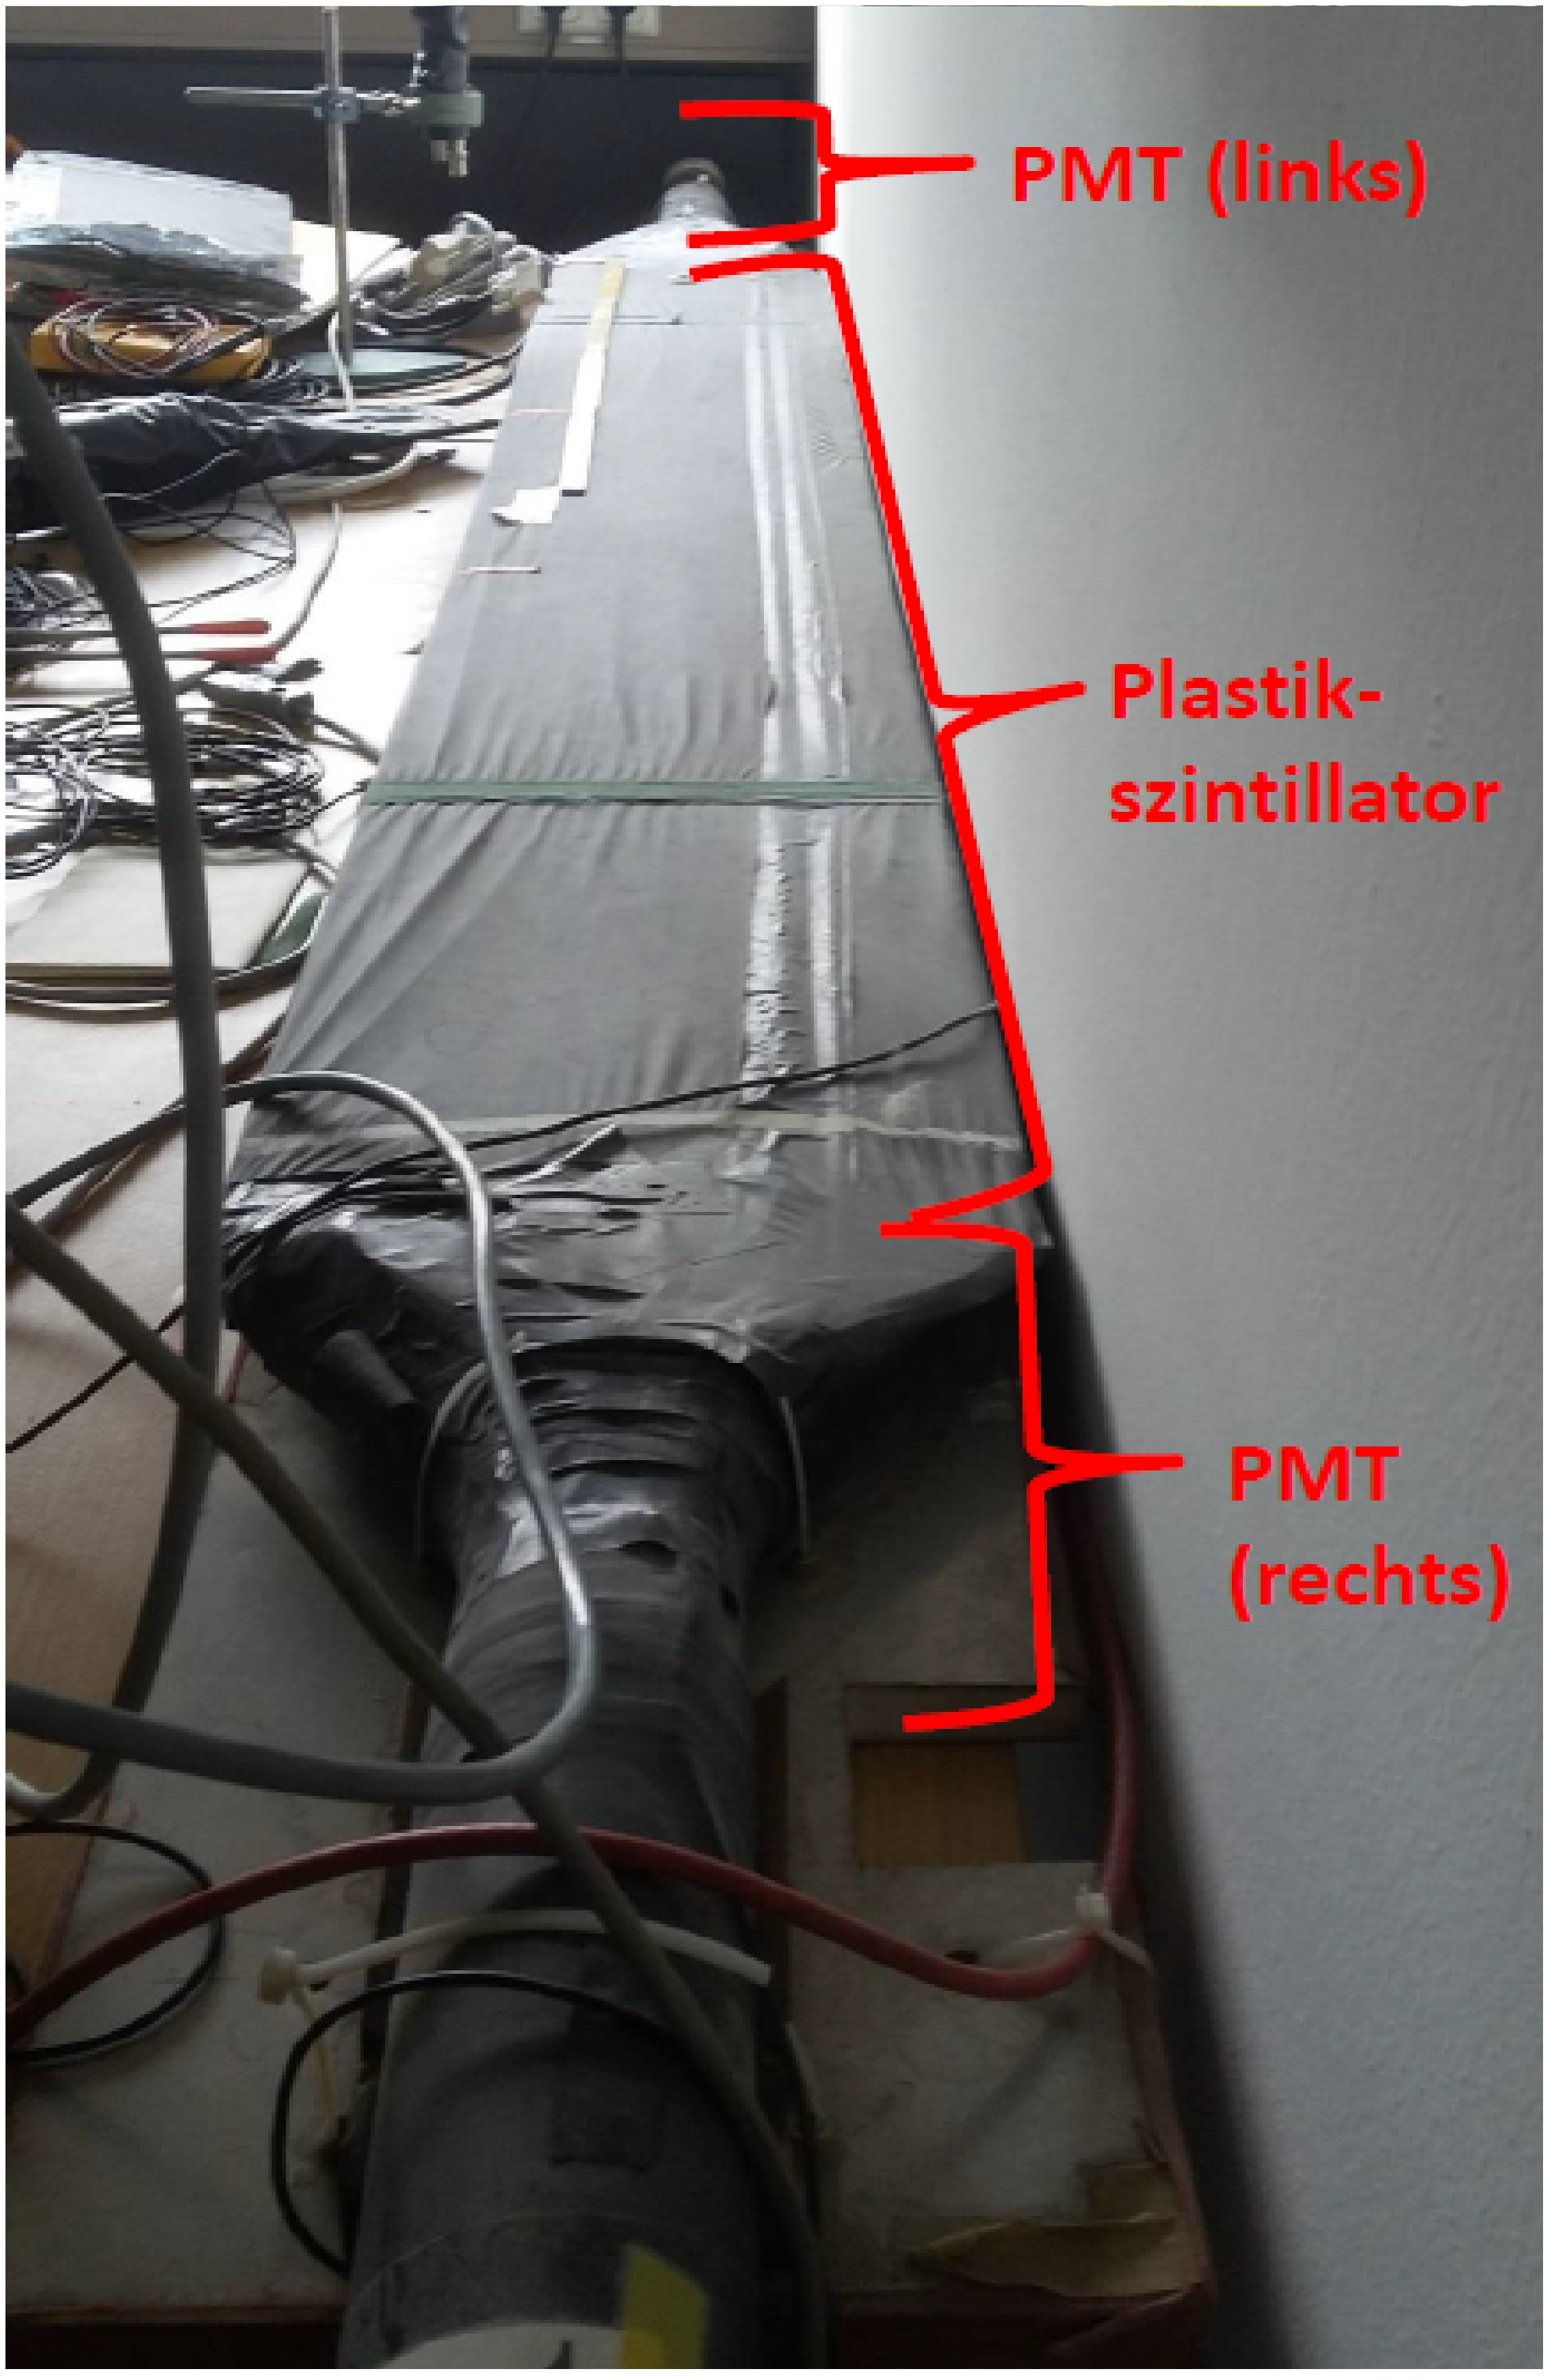
\includegraphics[width=1\textwidth]{Plots/Scintillator.jpg}
\end{subfigure}
\begin{subfigure}[h]{0.59\textwidth}
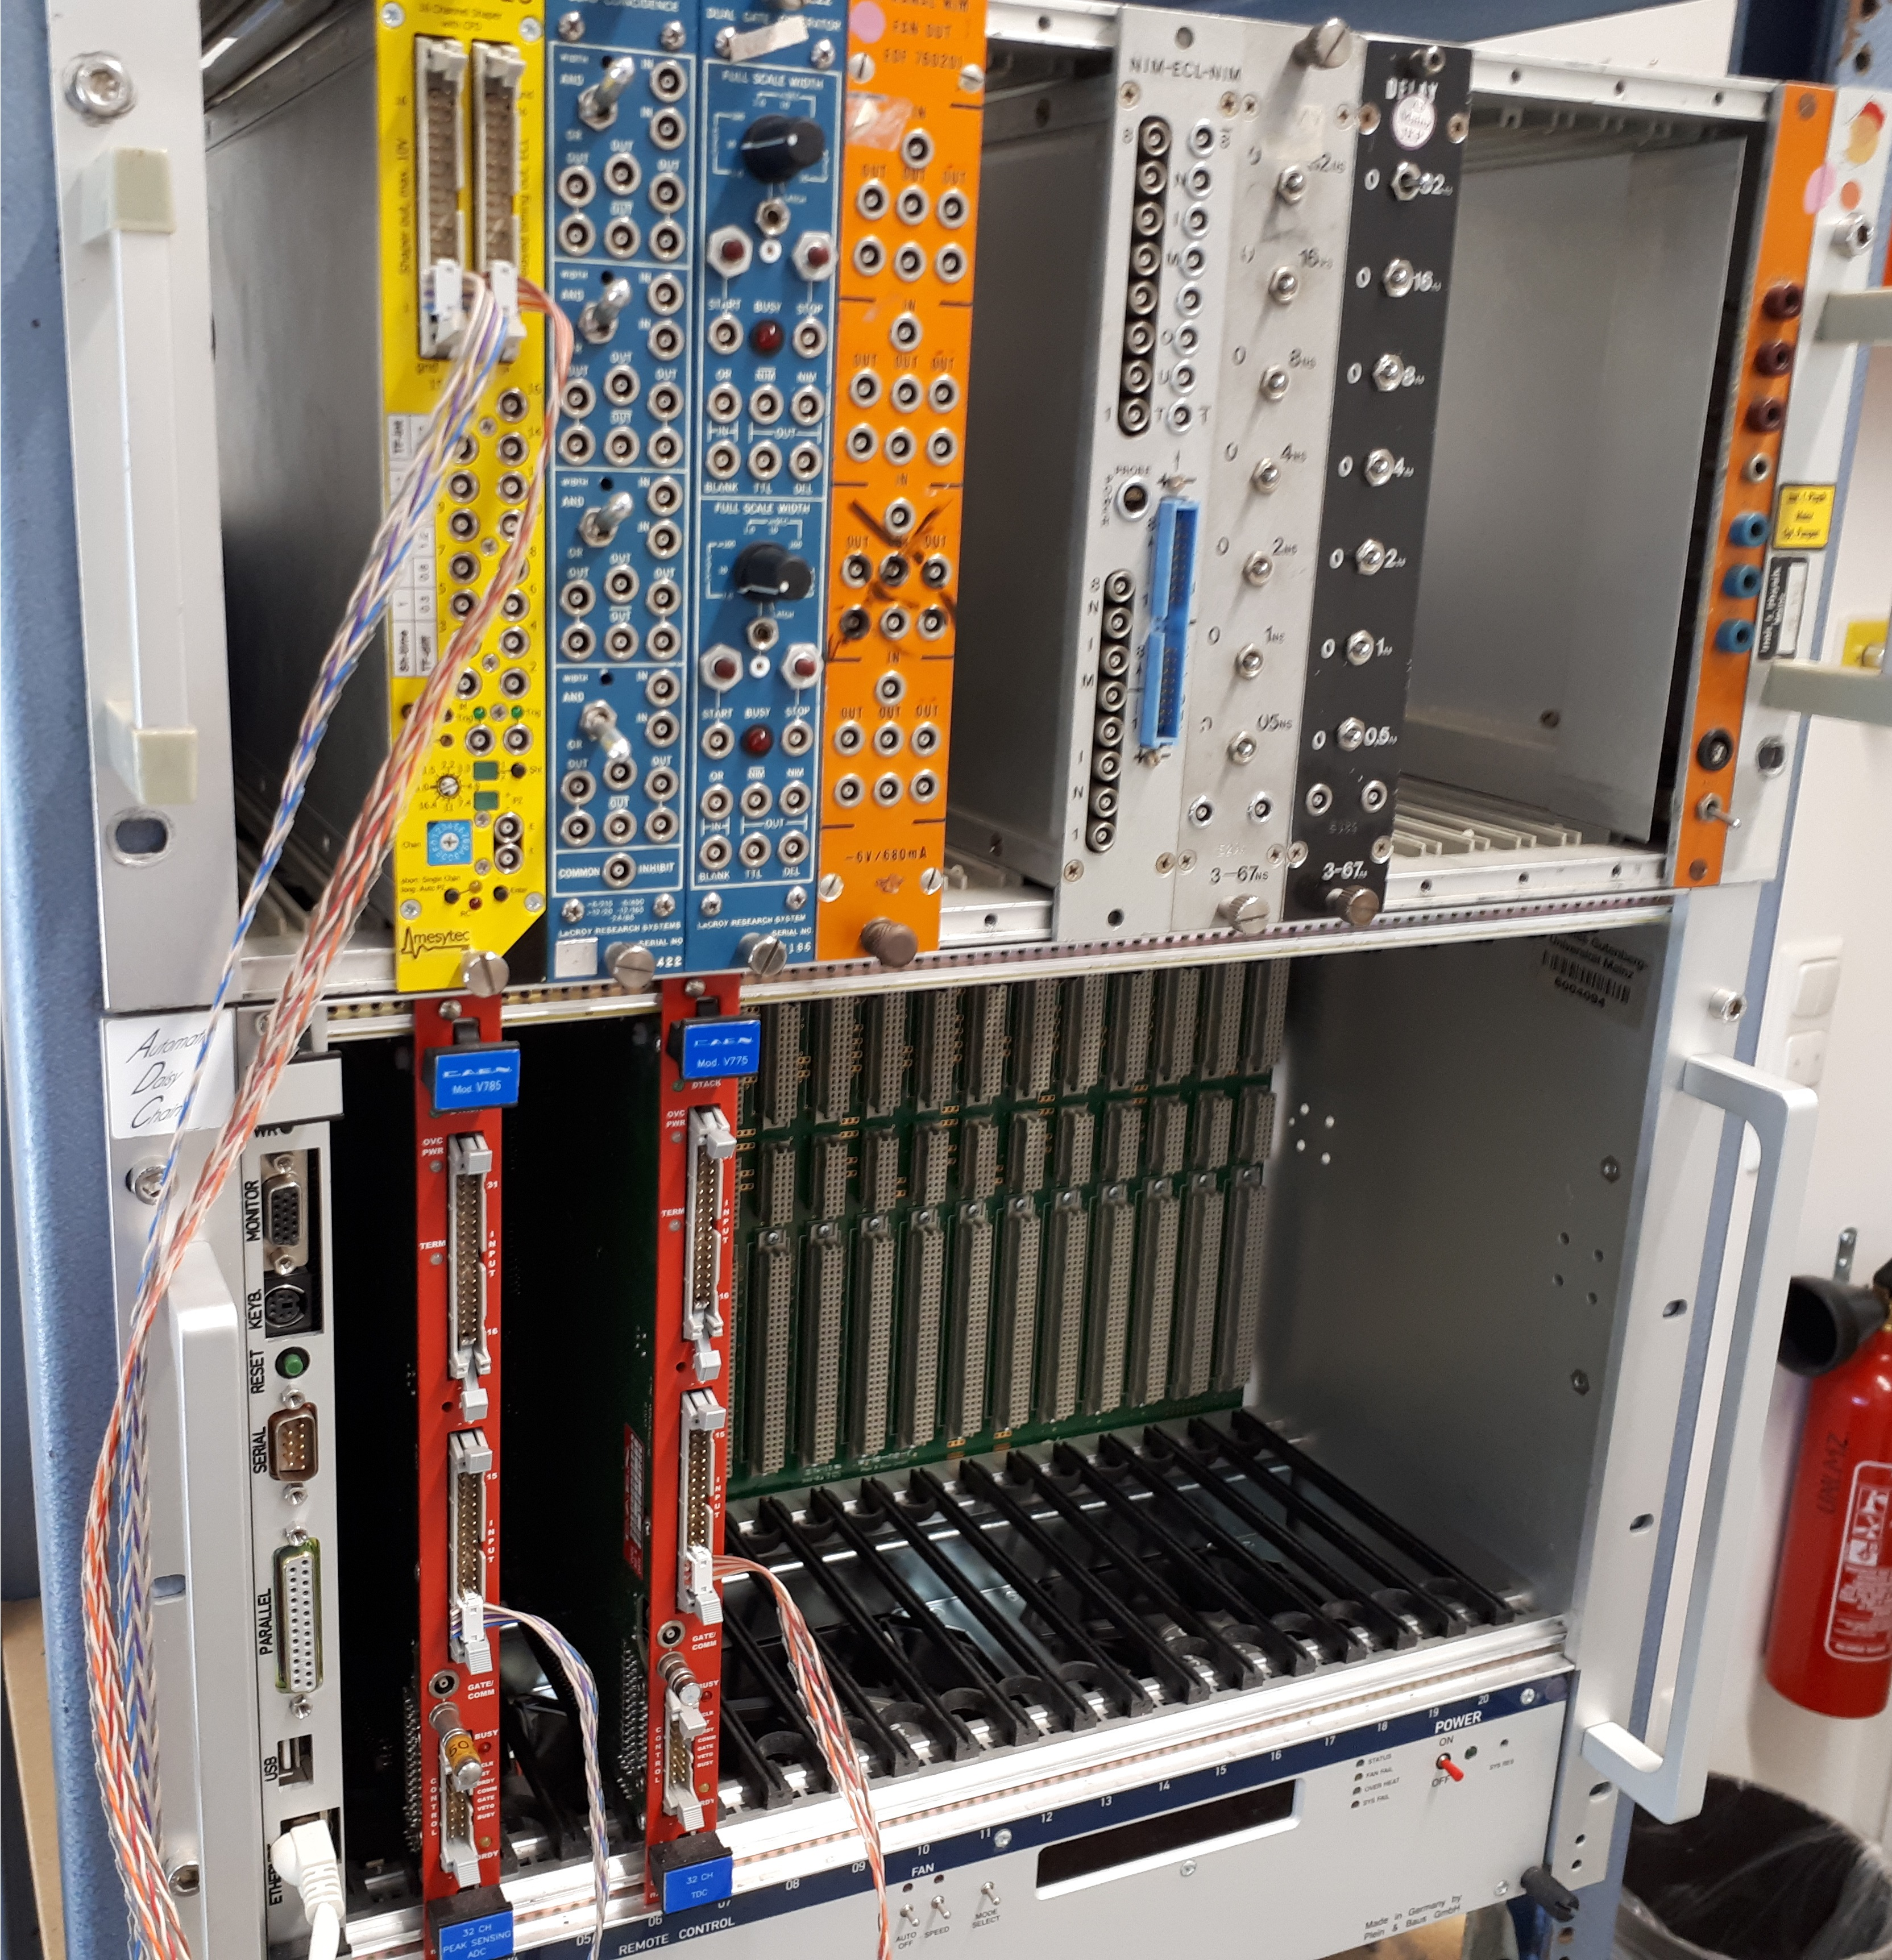
\includegraphics[width=1\textwidth]{Plots/Raw.jpg}
\end{subfigure}
\caption{Pictures of the set up. Scintillator and PMTs on the right \cite{script}. Data acquisition rack on the left without cabling. Declaration see figure \ref{fig:cabling}.}
\label{fig:setup}
\end{figure}

Both of the PMT outputs are connected with the MSCF-16 unit, the yellow one in figure \ref{fig:setup} and \ref{cabling}. The L labelled cable form the left PMT and the R labelled with an additional delay from the right one. Those Delay Boxes are just more cables the signal has to pass. From the MSCF-16 on the raw data will be delayed and passed to the analogue-to-digital converter (ADC) and time-to-digital converter (TDC) on the bottom of the pictures of the rack. And there it will be processed into the data we are working with later on. Another output leads over the third black cable to the Fan-In/-Out where the signal gets copied and passed to the Dual Gate Generator.

%%%%% Platz für mehr text :D # dont float mi floats 

\begin{figure}[H]
\centering
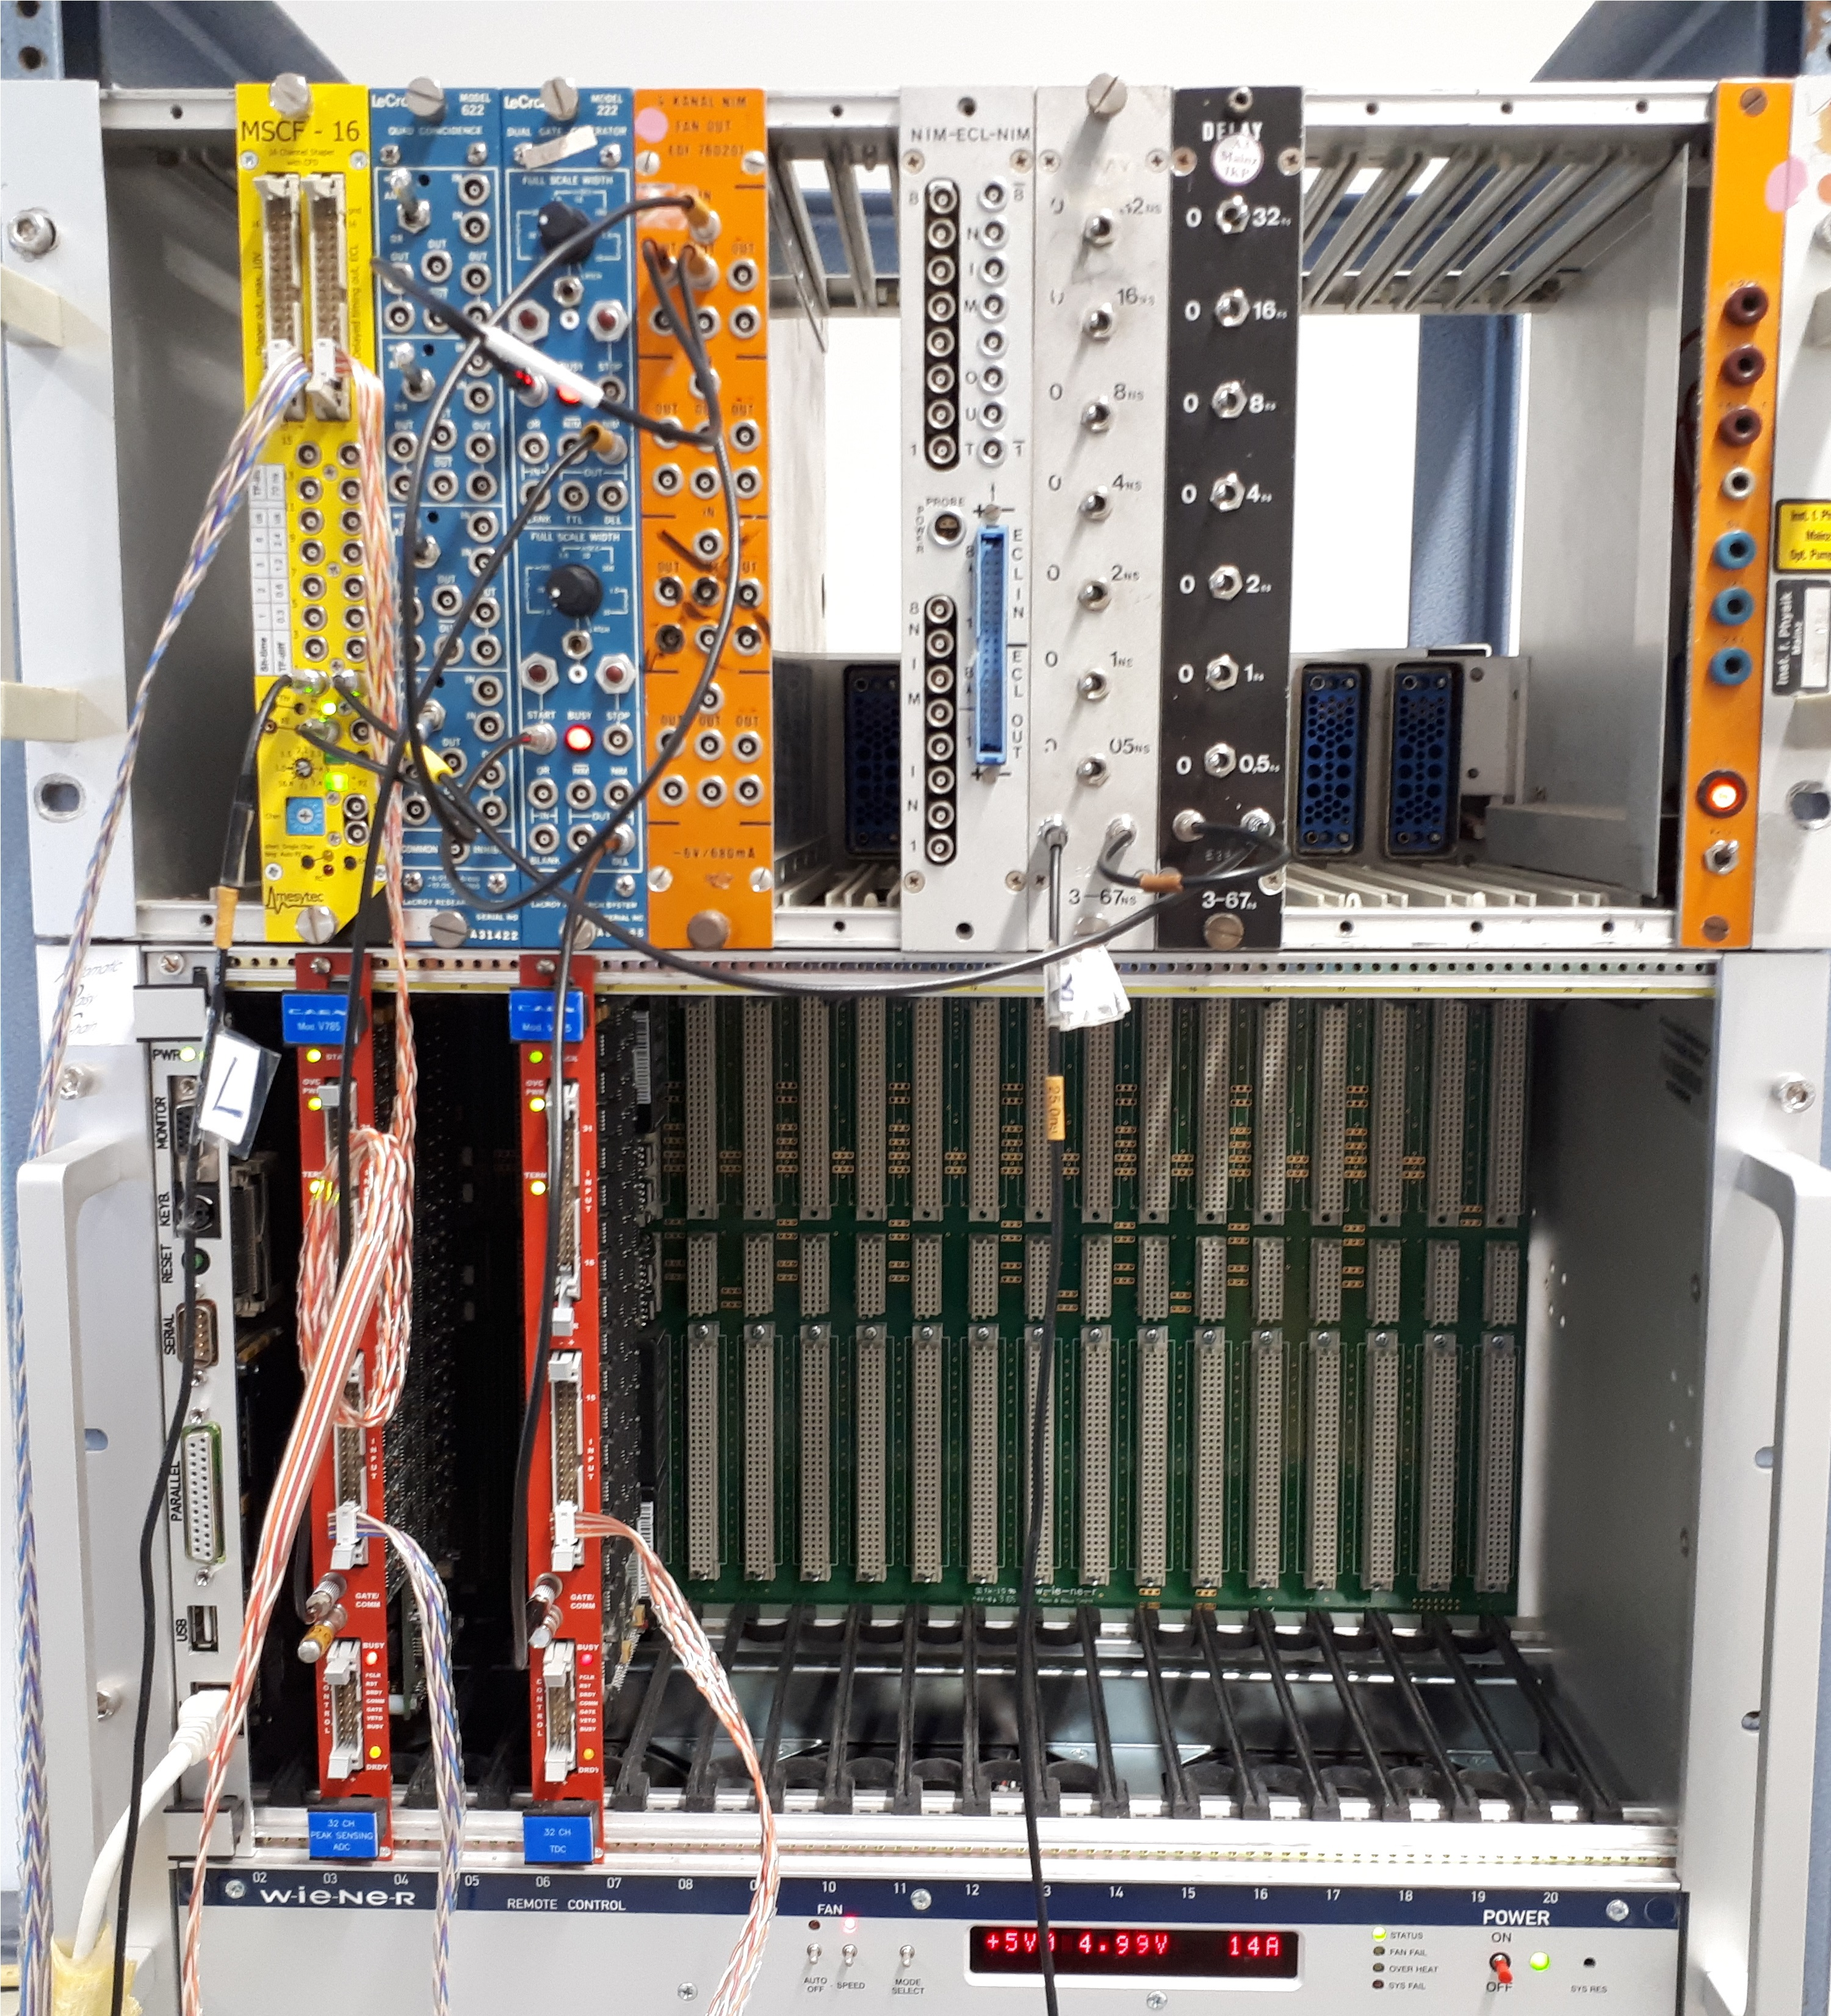
\includegraphics[width=1\textwidth]{Plots/Kabel2.jpg}
\caption{Data acquisition rack with cabling. Top left to right: MSCF-16, Quad Coincidence LeCroy 622 - not used, Dual Gate Generator LeCroy 222, Fan-In/-Out, NIM-ECL-NIM
module, two Delay Boxes.
Bottom: Gateway for PC connection, ADC, TDC.  }
\label{fig:cabling}
\end{figure}
%%%%%%%%%%%%%%%%%%%%%%%%%%%%%%%%%%%%% Kabel Schema aus Skript mit ins Bild paint'en?

The Gate Generators Delayed Output (DEL) produces a short signal for the TDC. This first signal starts the time measurement and gets stopped by the delayed signal of the MSCF-16. The length of the first triggering signal determines how long the second one will be measured. The ADC on the other hand receives a long signal from the gate generator. This leads to a good energy resolution but won't be necessary in this experiment.

%%% Description of how the data gets passed
\begin{figure}[H]
\centering
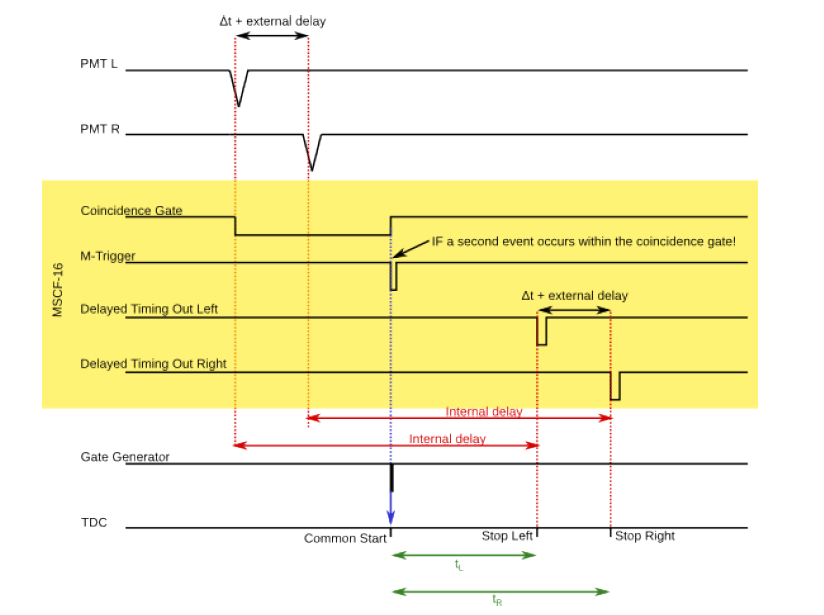
\includegraphics[width=1\textwidth]{Plots/Timing.png}
\caption{Schematic display on how the signals are passed between the components and what the TDC returns. \cite{script}}
\label{fig:timing}
\end{figure}

Now for a detailed description on what happens see figure \ref{fig:timing}. On top are the original signals the MSCF-16 receives. The signal from the right is delayed by the Delay Boxes. The first signal from the left PMT starts a coincidence gate. This is a variable time frame in which another signal has to appear to create a trigger which is used to start the time measurement. This helps to separate events and noise...
%%%%%%% WOZU ist denn dieses coincidence gate wirklich da?  
As explained above, the trigger signal is split in two at the Fan-In/-Out and processed in the gate generators for the special converter. In the TDC the delayed signal of the MSCF-16 then stops the time measurement. For us the time difference $t_R - t_L$ is of interest. This is proportional to the delay boxes delay and later on it will depend on where our radioactive sample is placed.

\subsection{Cosmic Muons} % aka Setup 2.0
% Cabling via NIM_ECL_NIM to the oszi
% no photos taken
% justierung des Spannungsverteilers

\begin{figure}[H]
\centering
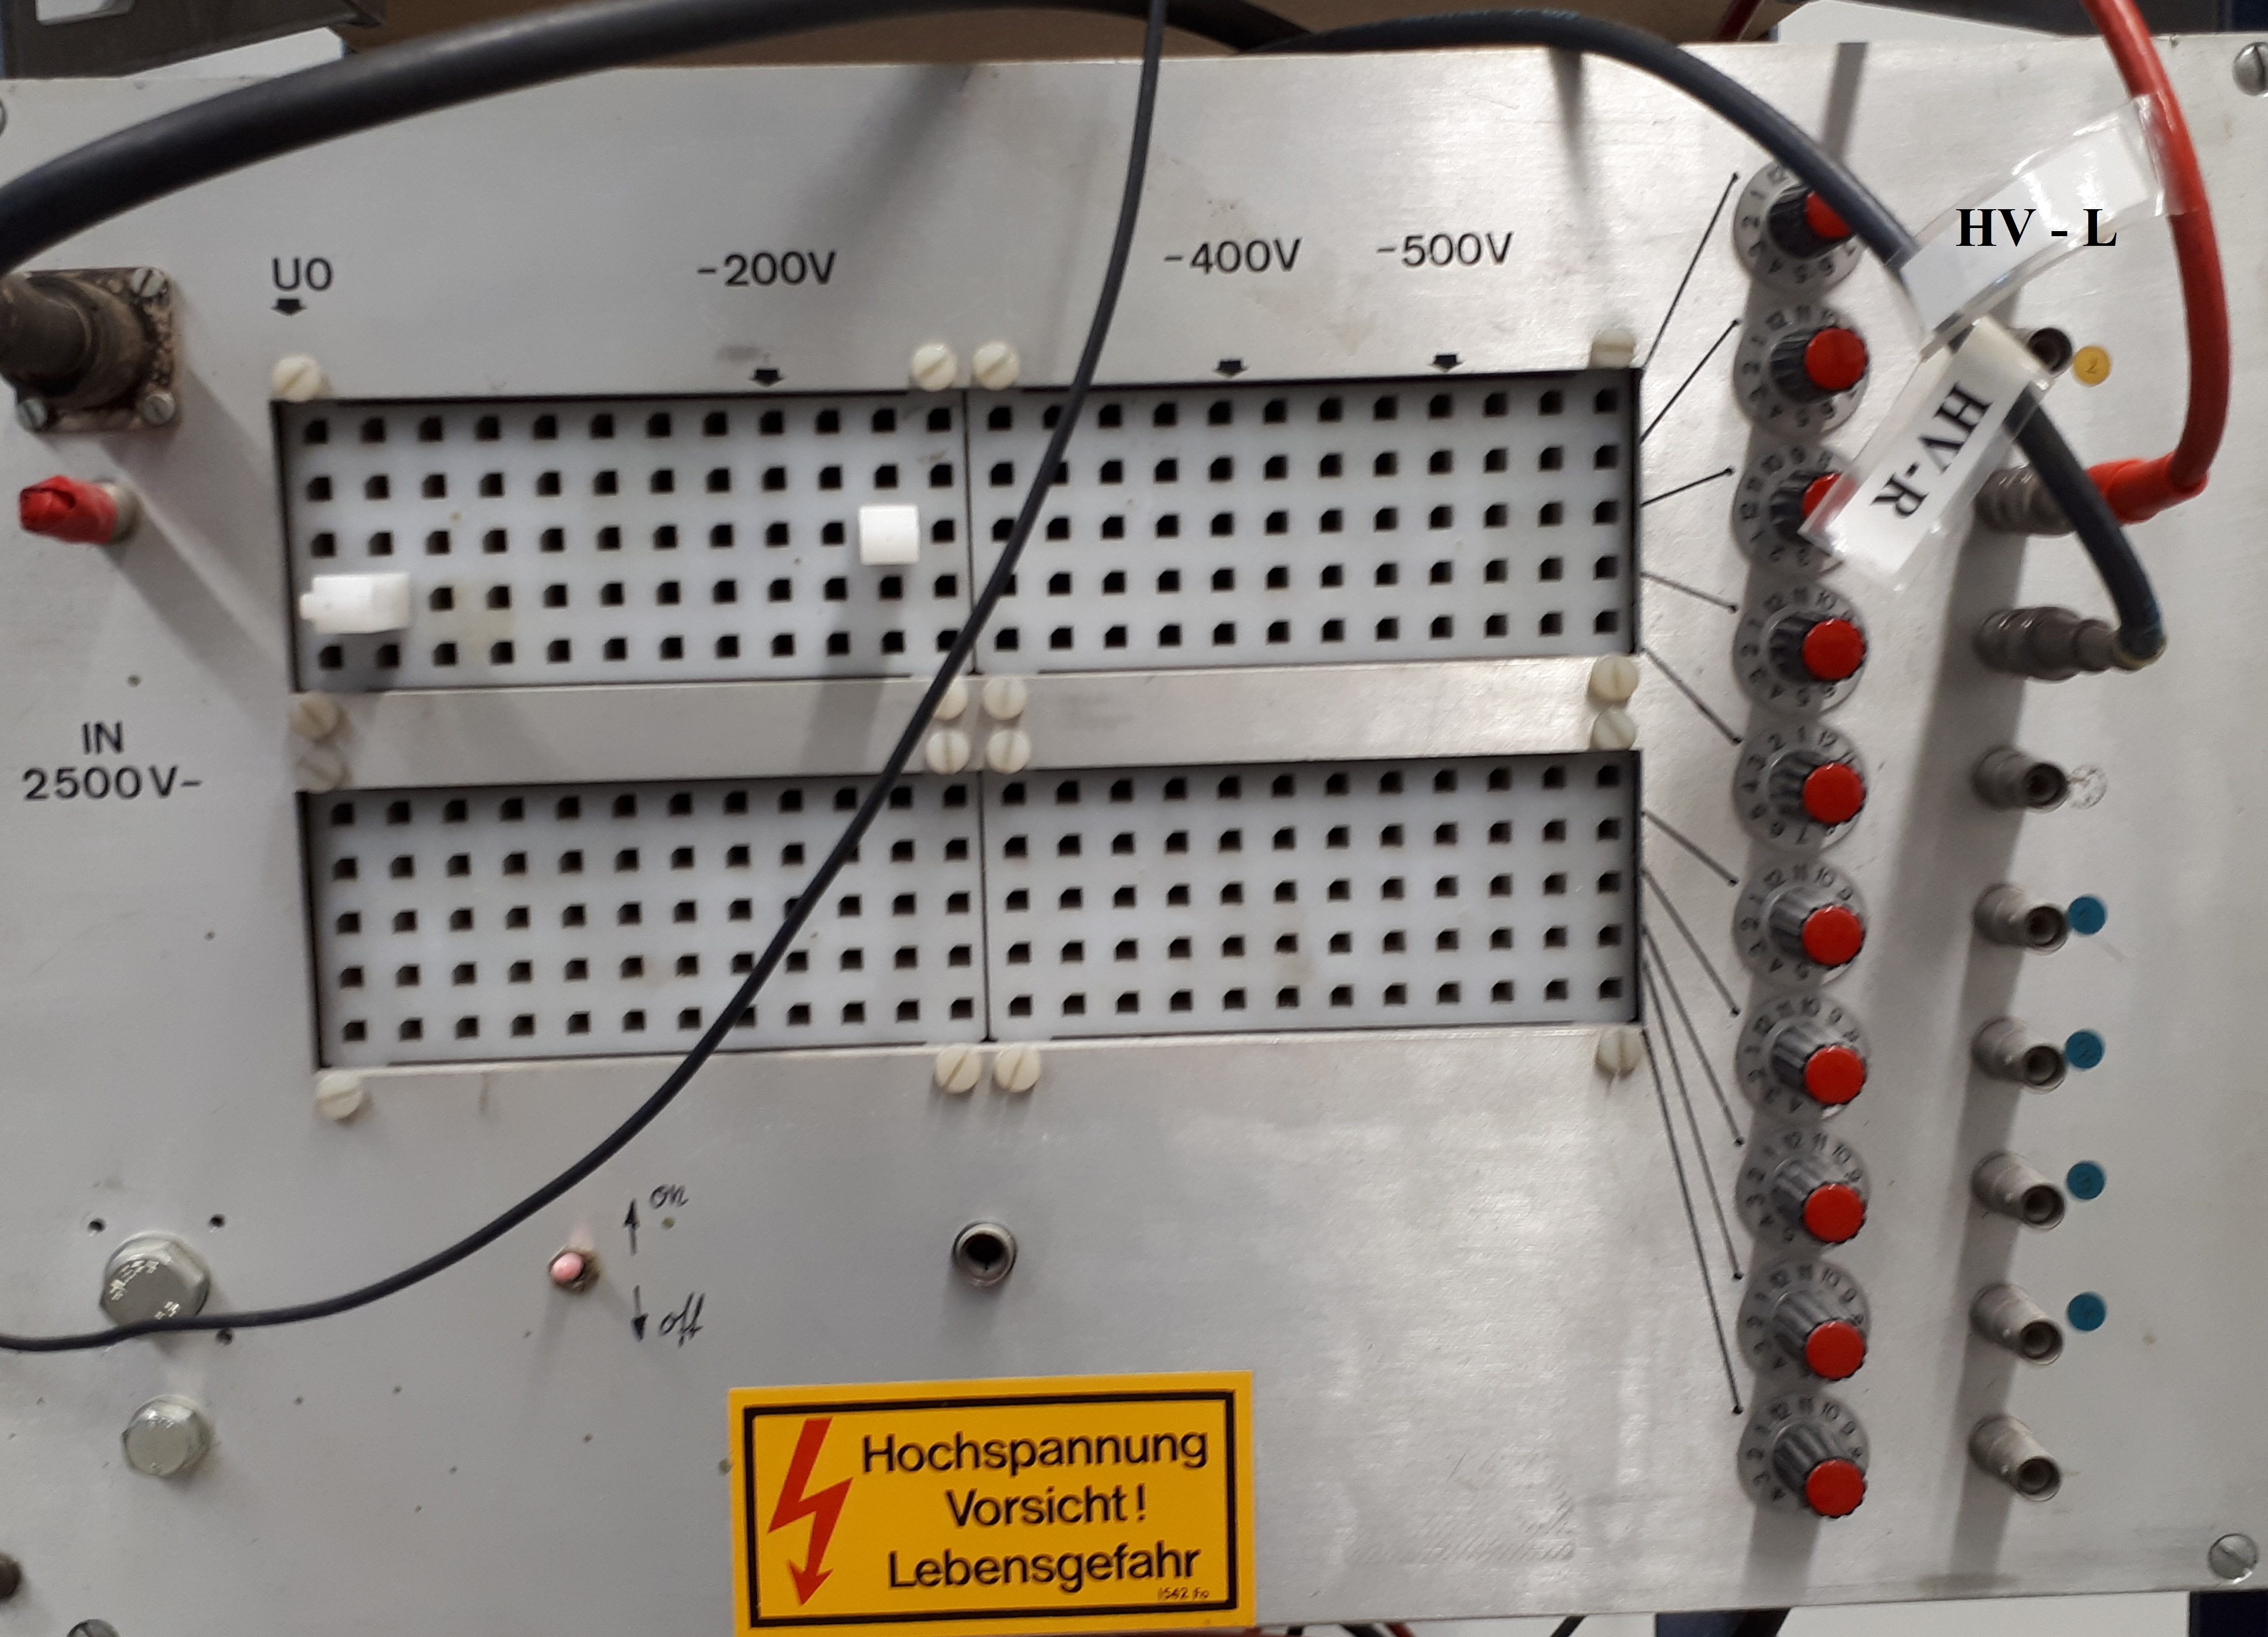
\includegraphics[width=1\textwidth]{Plots/Spannung.jpg}
\caption{Picture of the voltage distribution for similar PMT signals. HV-L (red) supplies the left PMT and HV-R (black) the right one.}
\label{fig:voltage}
\end{figure}


\subsection{Time calibration}\label{time}
For this chapter we placed a $^{207}Bi$ source on top of the scintillator. A folding yardstick was fasten on top. For the calibration we placed the source at $100cm$ which is the middle of the scintillator. This should result in equal time delay, if the Delay Boxes are not used and the same cables are used. To determine at which time unit the most events occurred each $50\ 000$ events were measured to create a histogram. This treatment stays the same for the following calibration and the determination of the speed of light c.

Because we have no value how many time units are equal to $1ns$, the calibration has to be done. We started with an offset of $32ns$ on the delay boxes, to ensure that the left PMT always starts the coincidence gate for consistency. By increasing the additional delay the time difference will rise too and therefore a proportionality will be visible.

Each data set of $50\ 000$ events is presented in the histograms in the Appendix \ref{appendix}. Each is fitted by the Gaussian function, where $\mu$ is the expected value, $\sigma$ the standard derivation, A the maximum amount at $\mu$ and b a constant off-set.
\begin{equation}
n(x) = A\cdot exp \left( -\frac{(x-\mu)^2}{2\sigma^2} \right) + b
\end{equation}

%%%%  fit


\subsection{Speed of light measurement}\label{c determination}

%%% plot für 20 cm ist nicht im appendix
%%% Fehlerquelle: Kabellängen 

%%% refractive index ca. 1.58 \cite{refractive index}
\section{Appendix}\label{appendix}
\subsection{Time calibration}
\begin{figure}[H]
\centering
\medskip
\begin{subfigure}{0.48\textwidth}
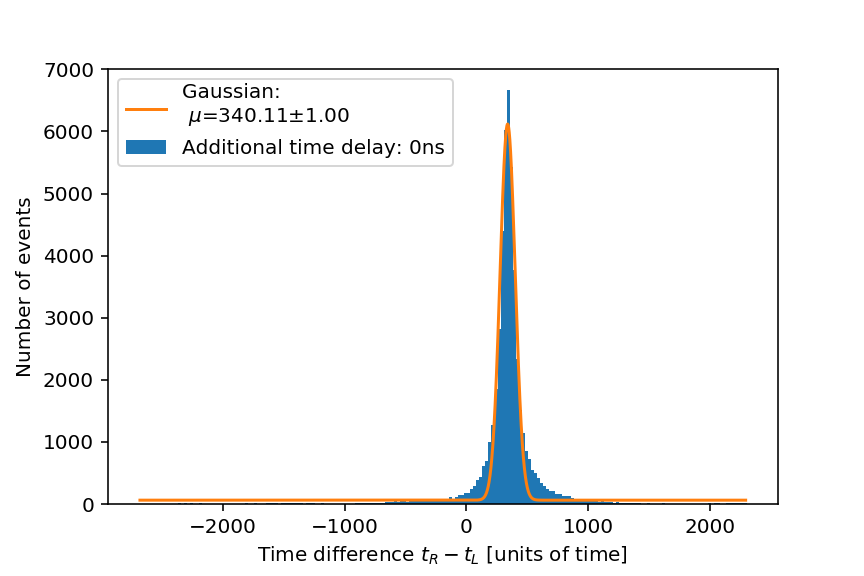
\includegraphics[width=\linewidth]{Plots/Time/0ns.png}
\end{subfigure}
\begin{subfigure}[c]{0.48\linewidth}
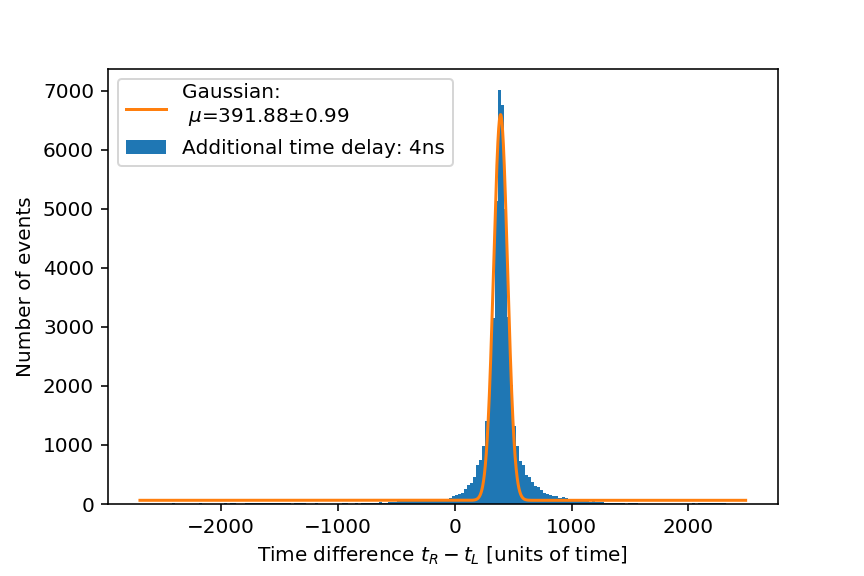
\includegraphics[width=\linewidth]{Plots/Time/4ns.png}
\end{subfigure}

\medskip
\begin{subfigure}{0.48\textwidth}
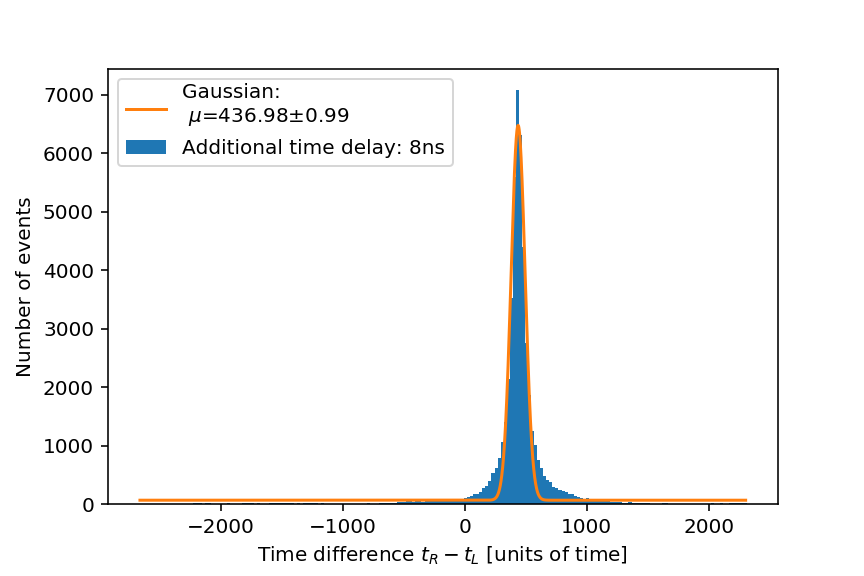
\includegraphics[width=\linewidth]{Plots/Time/8ns.png}
\end{subfigure}
\begin{subfigure}[c]{0.48\linewidth}
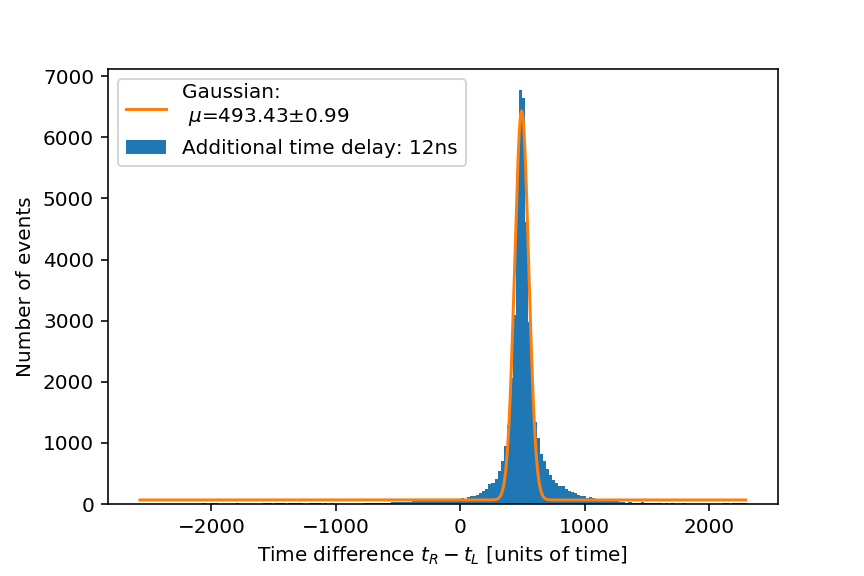
\includegraphics[width=\linewidth]{Plots/Time/12ns.png}
\end{subfigure}

\medskip
\begin{subfigure}{0.48\textwidth}
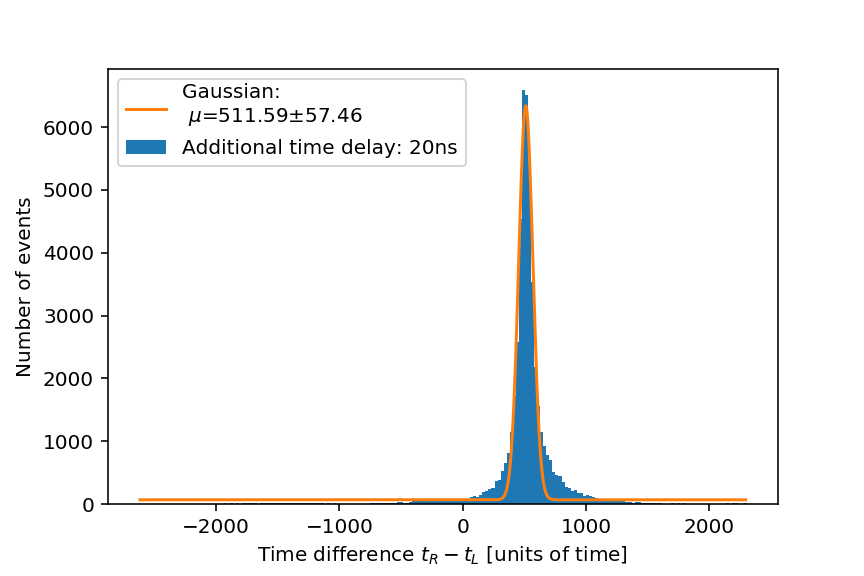
\includegraphics[width=\linewidth]{Plots/Time/20ns.png}
\end{subfigure}
\begin{subfigure}[c]{0.48\linewidth}
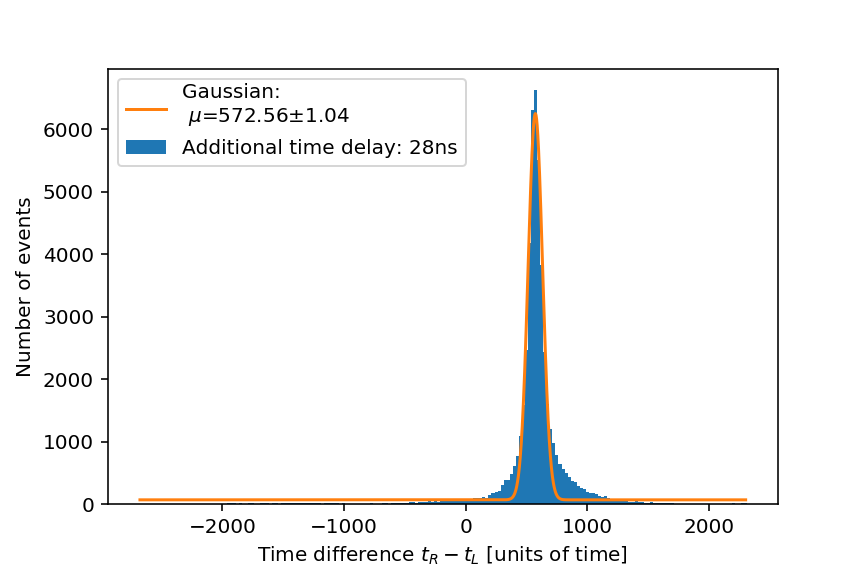
\includegraphics[width=\linewidth]{Plots/Time/28ns.png}
\end{subfigure}
\caption{Histograms for the time calibration in chapter \ref{time}. Part I }
\end{figure}

\begin{figure}[H]
\centering
\medskip
\begin{subfigure}{0.48\textwidth}
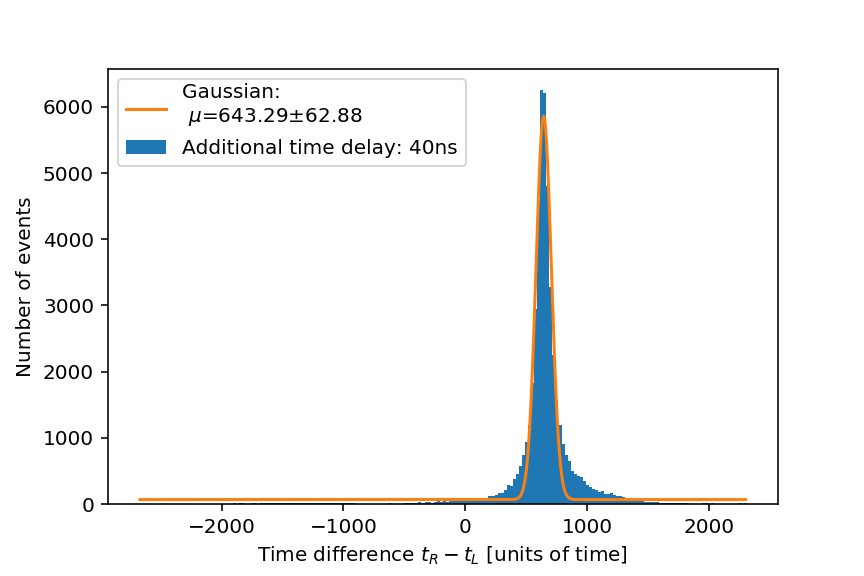
\includegraphics[width=\linewidth]{Plots/Time/40ns.png}
\end{subfigure}
\begin{subfigure}[c]{0.48\linewidth}
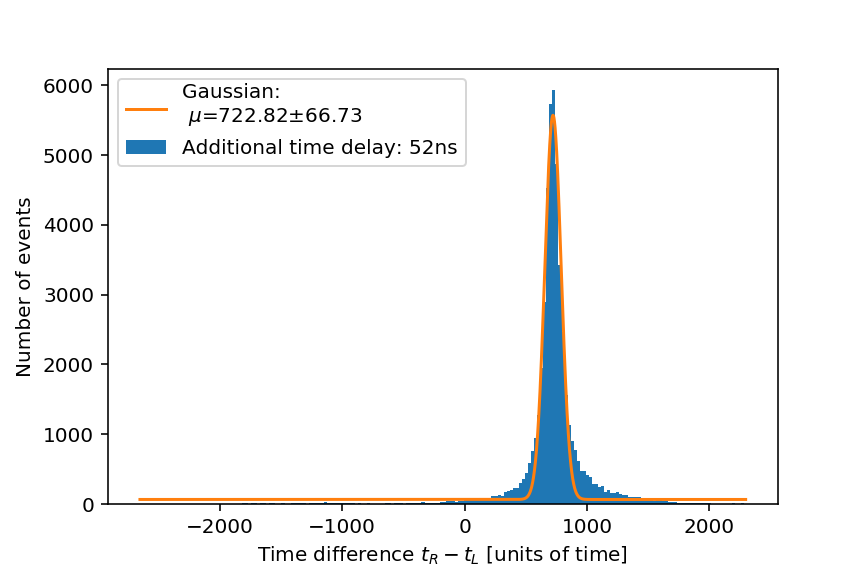
\includegraphics[width=\linewidth]{Plots/Time/52ns.png}
\end{subfigure}

\medskip
\begin{subfigure}{0.48\textwidth}
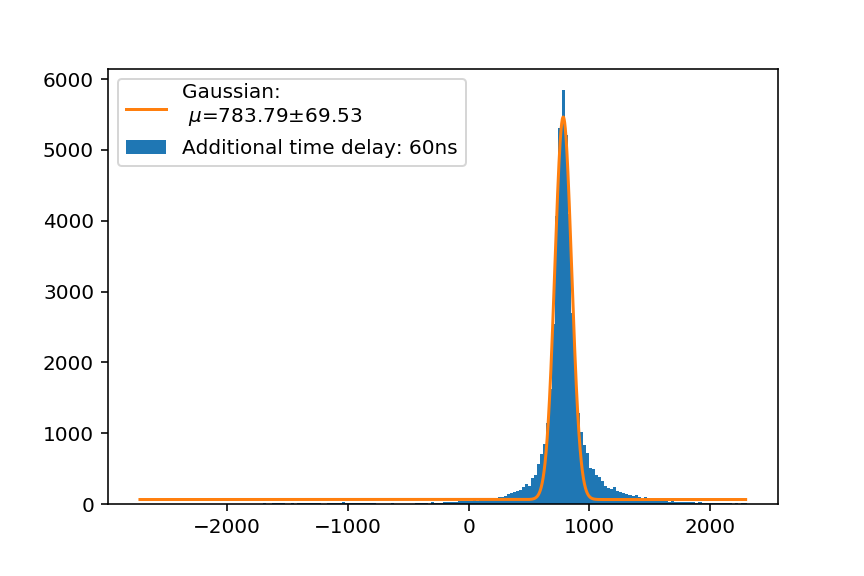
\includegraphics[width=\linewidth]{Plots/Time/60ns.png}
\end{subfigure}
\begin{subfigure}[c]{0.48\linewidth}
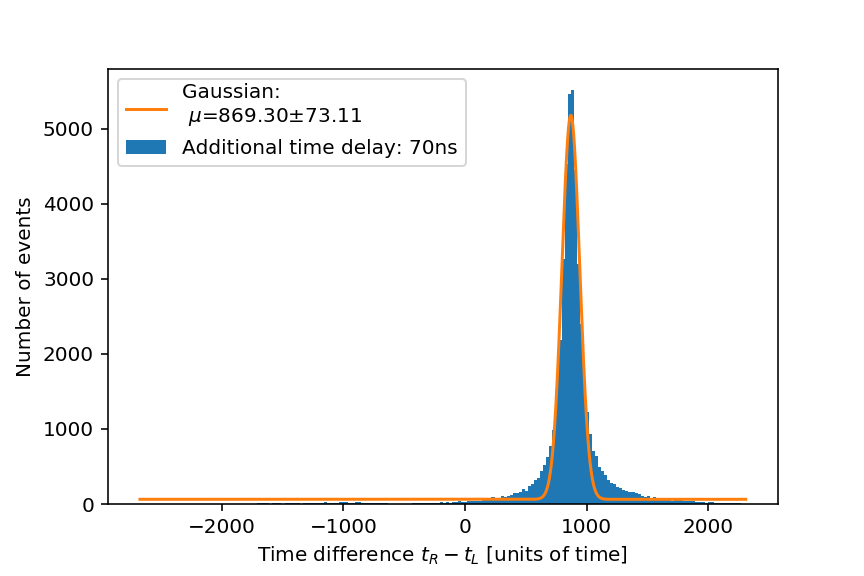
\includegraphics[width=\linewidth]{Plots/Time/70ns.png}
\end{subfigure}

\medskip
\begin{subfigure}{0.48\textwidth}
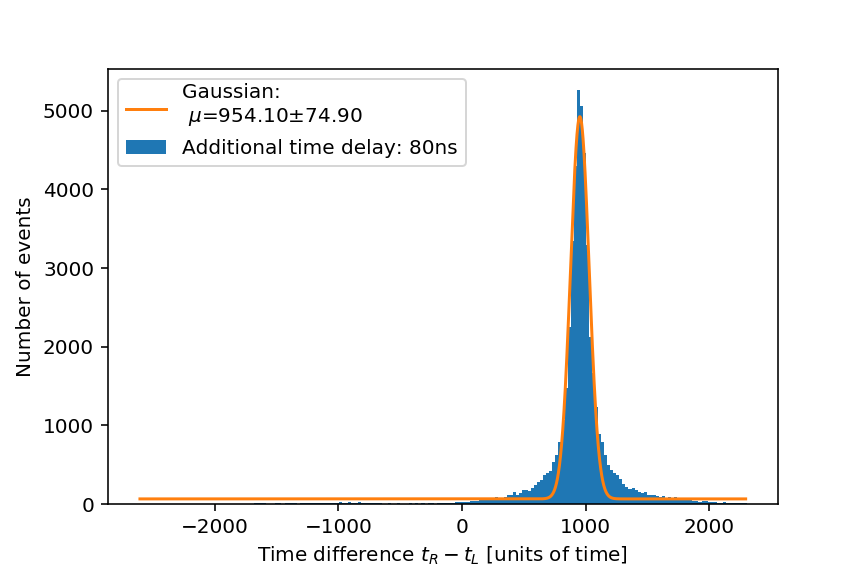
\includegraphics[width=\linewidth]{Plots/Time/80ns.png}
\end{subfigure}
\begin{subfigure}[c]{0.48\linewidth}
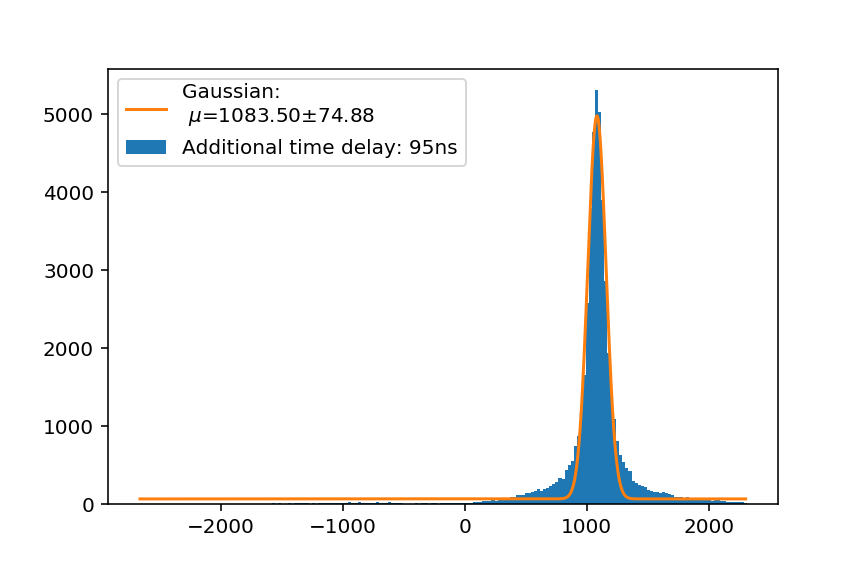
\includegraphics[width=\linewidth]{Plots/Time/95ns.png}
\end{subfigure}
\caption{Histograms for the time calibration in chapter \ref{time}. Part II }
\end{figure}


\subsection{Speed of light}
\begin{figure}[H]
\centering
\medskip
\begin{subfigure}{0.48\textwidth}
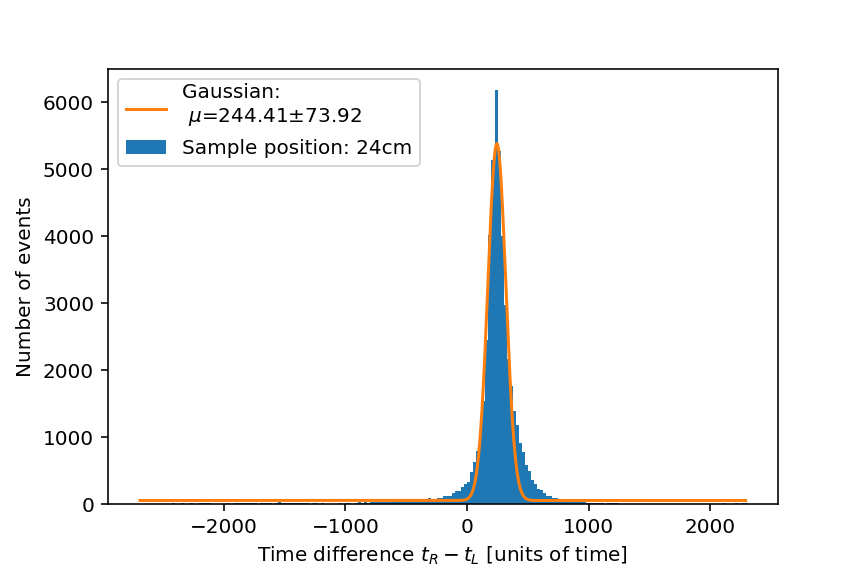
\includegraphics[width=\linewidth]{Plots/Pos/24cm.png}
\end{subfigure}
\begin{subfigure}[c]{0.48\linewidth}
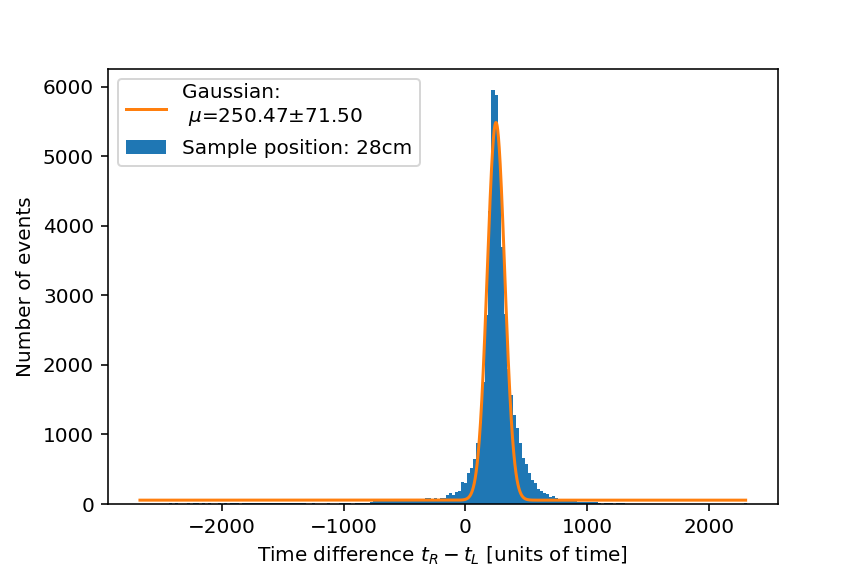
\includegraphics[width=\linewidth]{Plots/Pos/28cm.png}
\end{subfigure}

\medskip
\begin{subfigure}{0.48\textwidth}
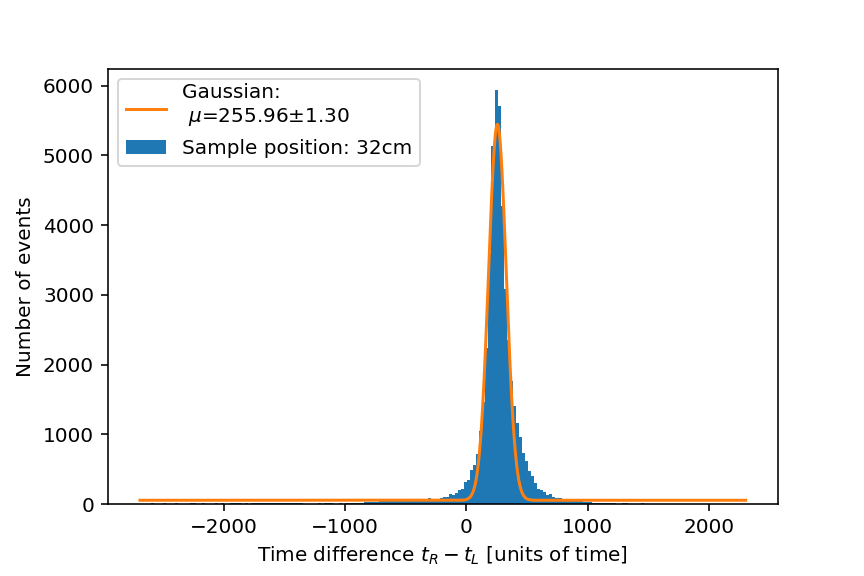
\includegraphics[width=\linewidth]{Plots/Pos/32cm.png}
\end{subfigure}
\begin{subfigure}[c]{0.48\linewidth}
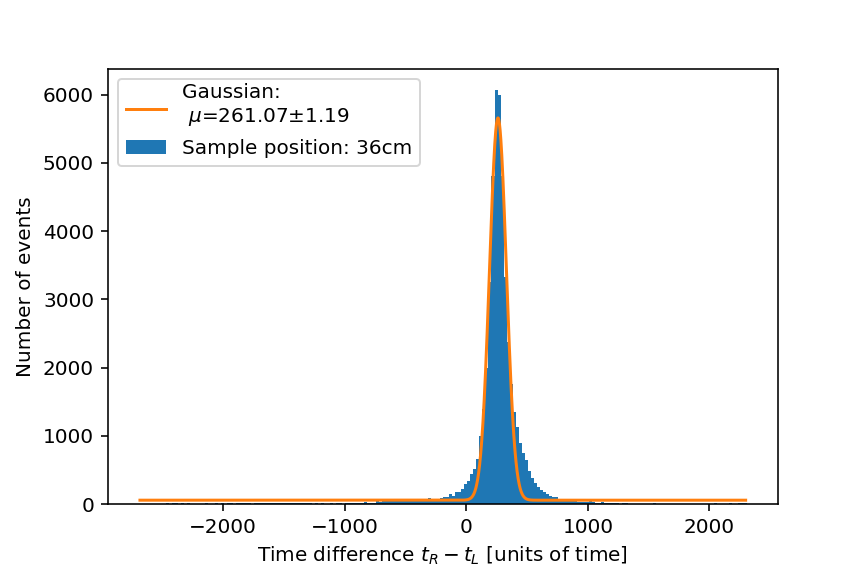
\includegraphics[width=\linewidth]{Plots/Pos/36cm.png}
\end{subfigure}

\medskip
\begin{subfigure}{0.48\textwidth}
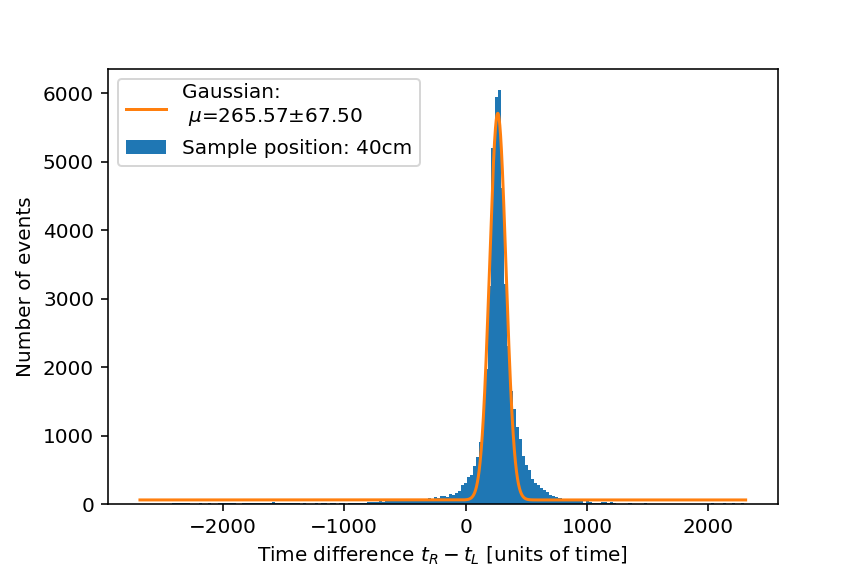
\includegraphics[width=\linewidth]{Plots/Pos/40cm.png}
\end{subfigure}
\begin{subfigure}[c]{0.48\linewidth}
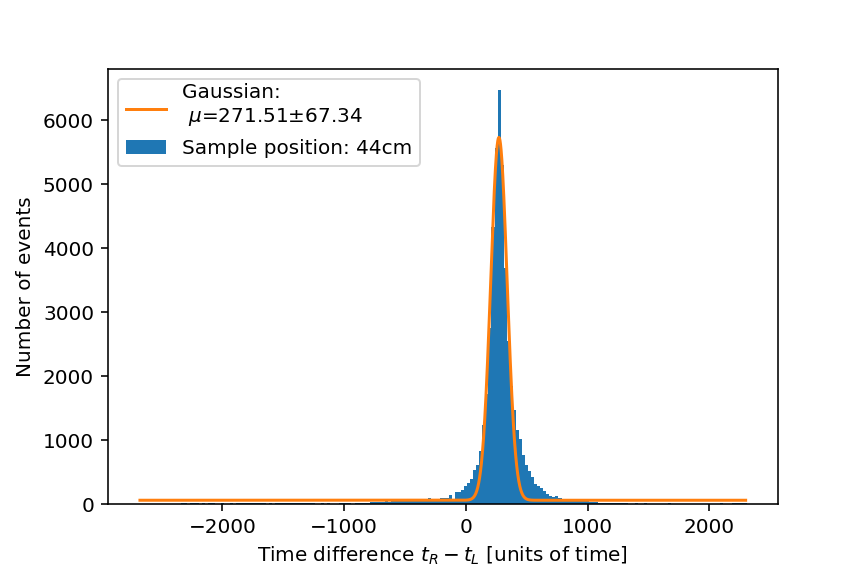
\includegraphics[width=\linewidth]{Plots/Pos/44cm.png}
\end{subfigure}

\medskip
\begin{subfigure}{0.48\textwidth}
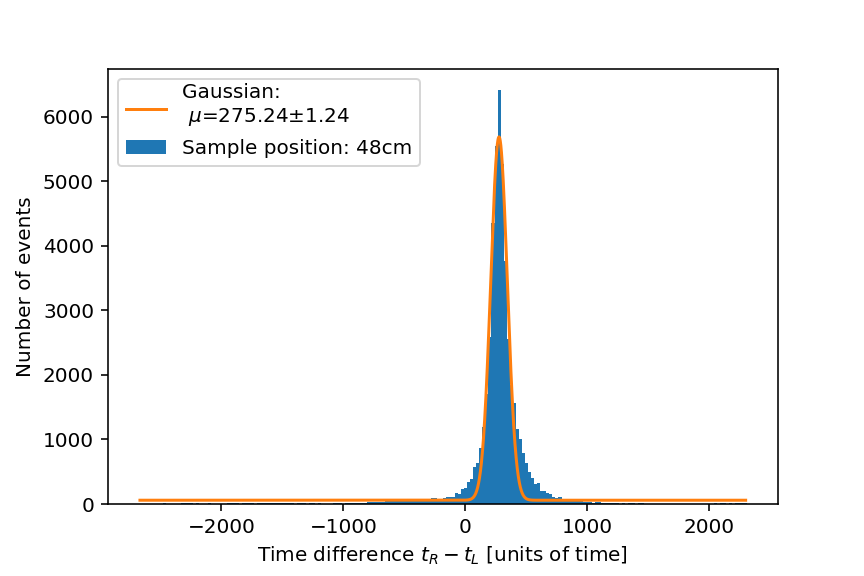
\includegraphics[width=\linewidth]{Plots/Pos/48cm.png}
\end{subfigure}
\begin{subfigure}[c]{0.48\linewidth}
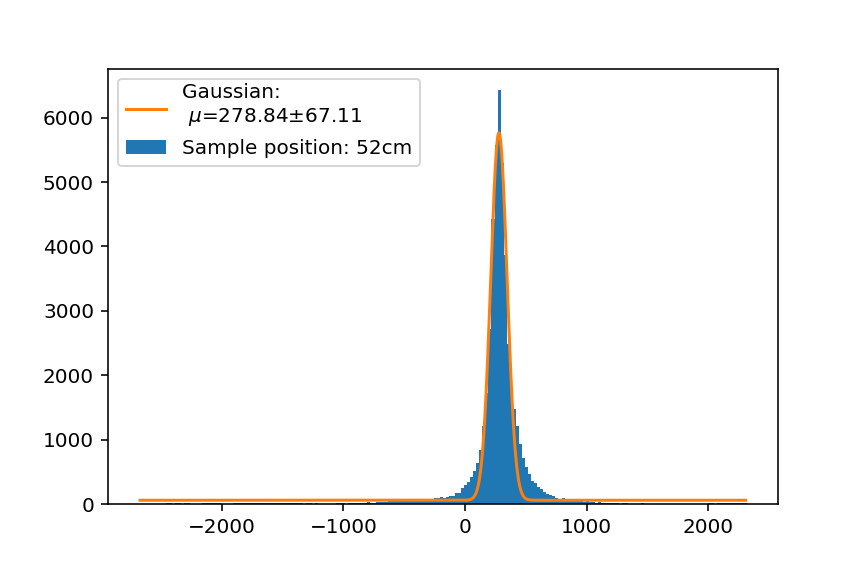
\includegraphics[width=\linewidth]{Plots/Pos/52cm.png}
\end{subfigure}
\caption{Histograms for the c calculation in chapter \ref{c determination}. Part I }
\end{figure}

\begin{figure}[H]
\centering
\medskip
\begin{subfigure}{0.48\textwidth}
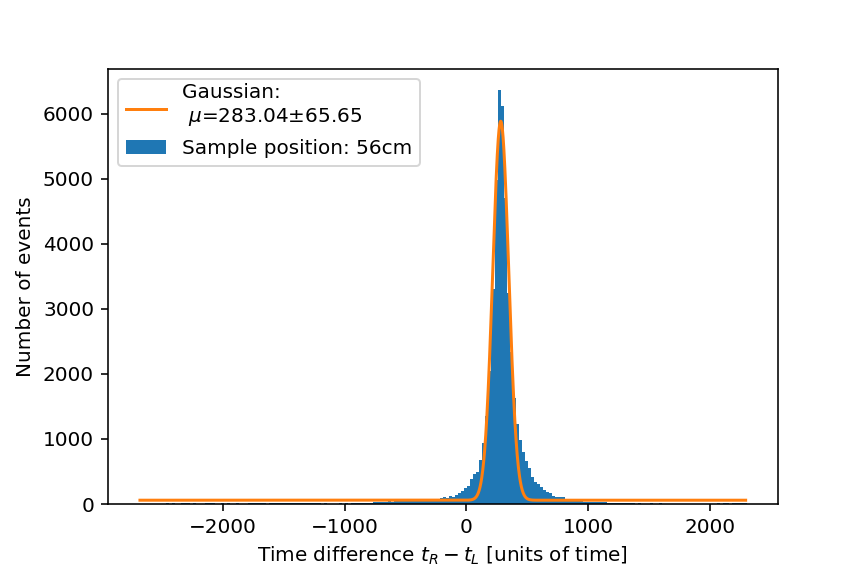
\includegraphics[width=\linewidth]{Plots/Pos/56cm.png}
\end{subfigure}
\begin{subfigure}[c]{0.48\linewidth}
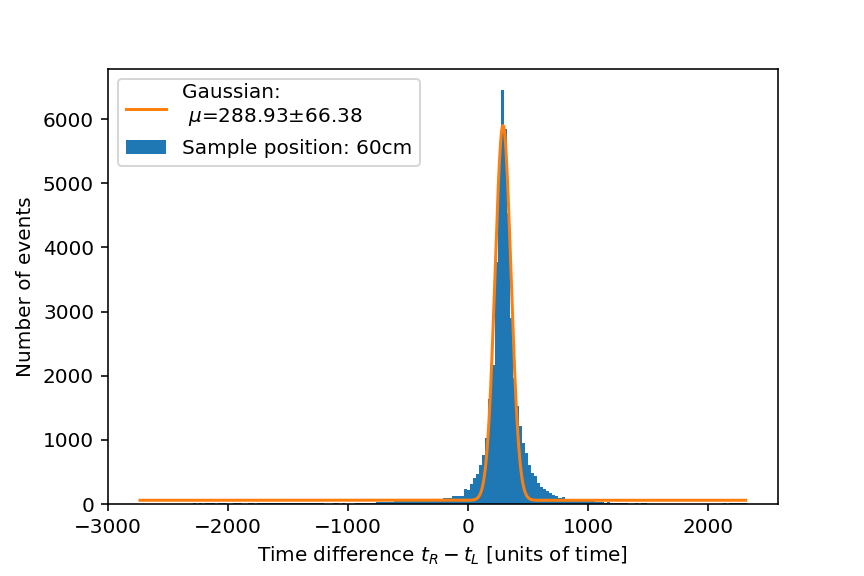
\includegraphics[width=\linewidth]{Plots/Pos/60cm.png}
\end{subfigure}

\medskip
\begin{subfigure}{0.48\textwidth}
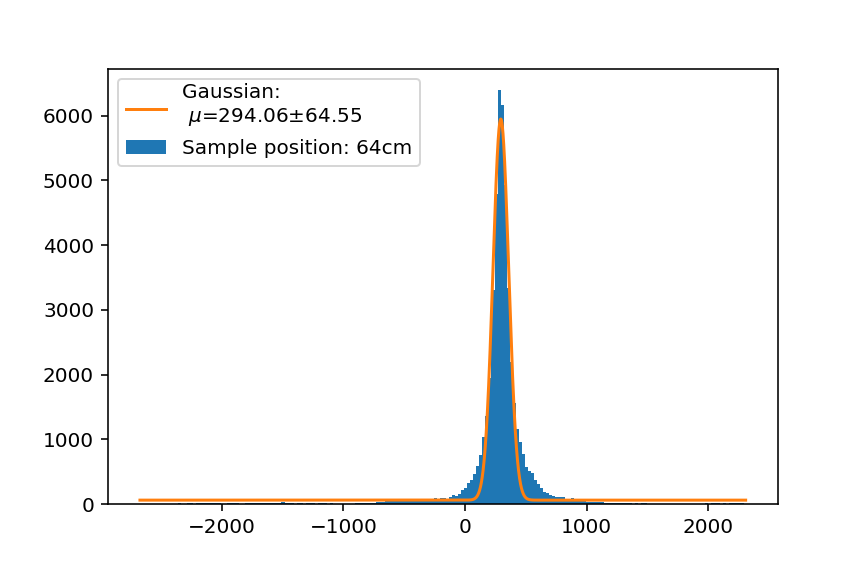
\includegraphics[width=\linewidth]{Plots/Pos/64cm.png}
\end{subfigure}
\begin{subfigure}[c]{0.48\linewidth}
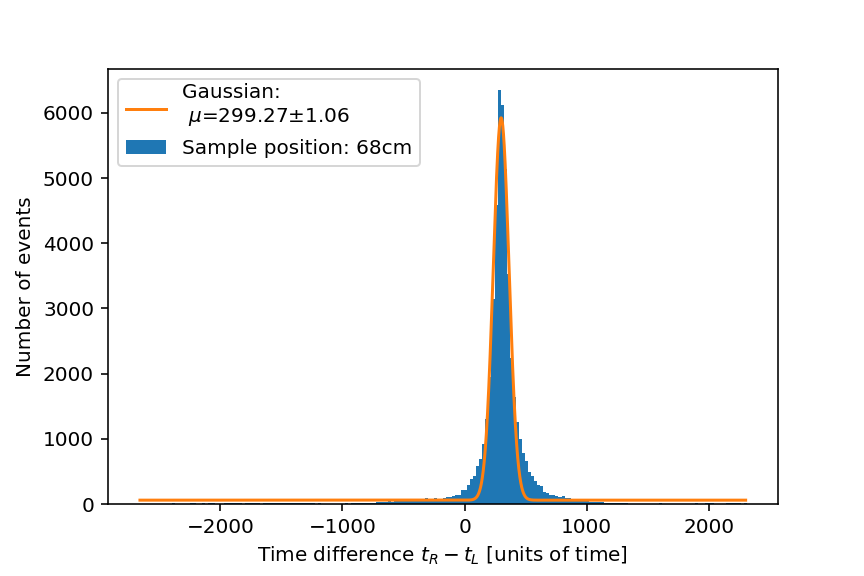
\includegraphics[width=\linewidth]{Plots/Pos/68cm.png}
\end{subfigure}

\medskip
\begin{subfigure}{0.48\textwidth}
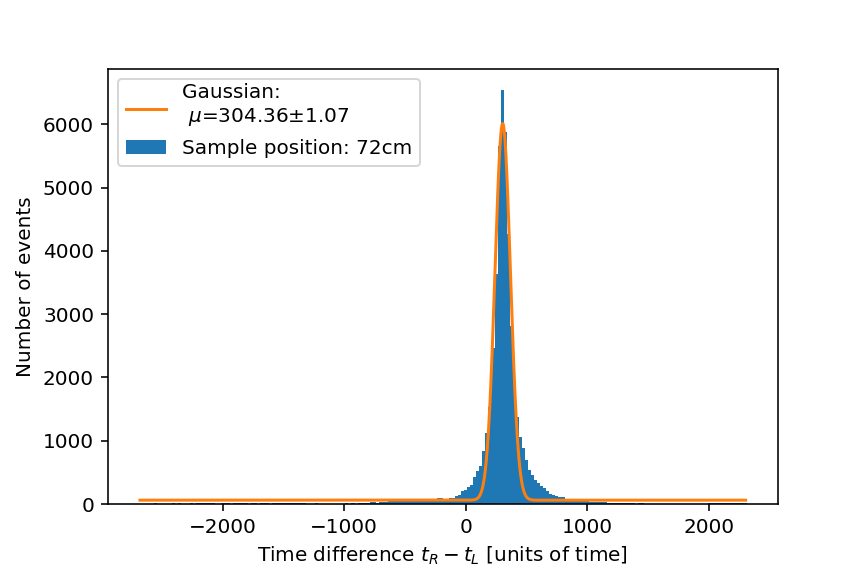
\includegraphics[width=\linewidth]{Plots/Pos/72cm.png}
\end{subfigure}
\begin{subfigure}[c]{0.48\linewidth}
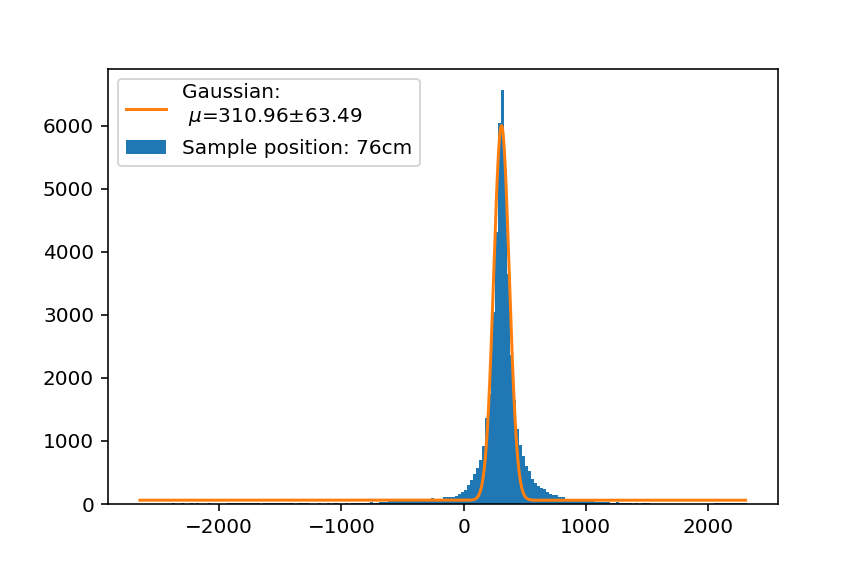
\includegraphics[width=\linewidth]{Plots/Pos/76cm.png}
\end{subfigure}

\medskip
\begin{subfigure}{0.48\textwidth}
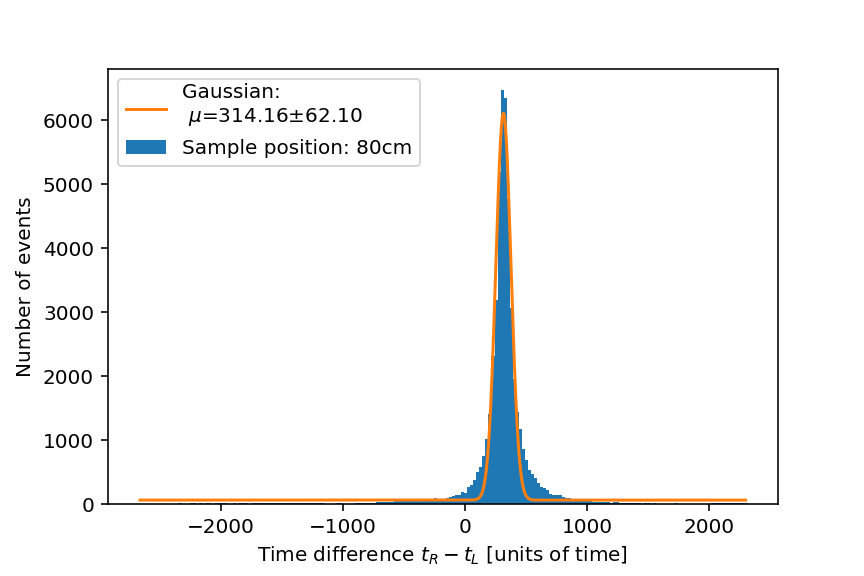
\includegraphics[width=\linewidth]{Plots/Pos/80cm.png}
\end{subfigure}
\begin{subfigure}[c]{0.48\linewidth}
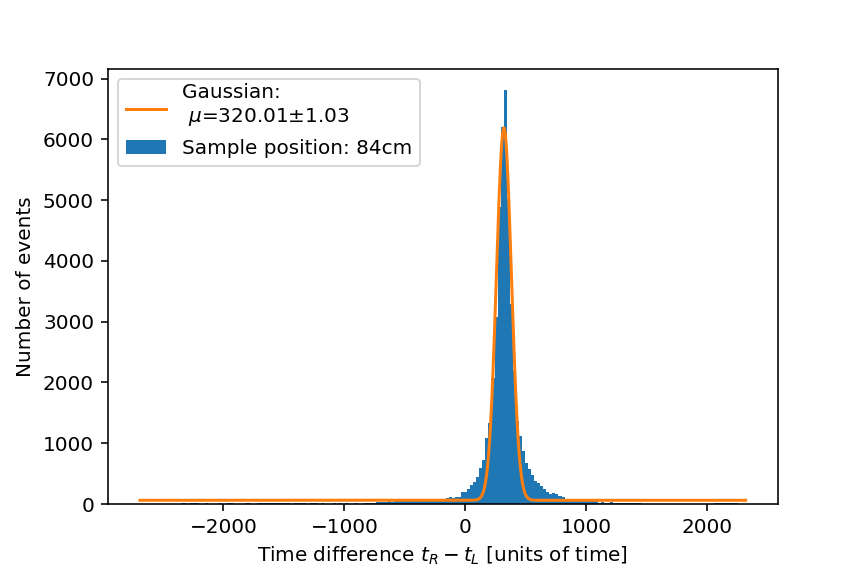
\includegraphics[width=\linewidth]{Plots/Pos/84cm.png}
\end{subfigure}
\caption{Histograms for the c calculation in chapter \ref{c determination}. Part II }
\end{figure}

\begin{figure}[H]
\centering
\medskip
\begin{subfigure}{0.48\textwidth}
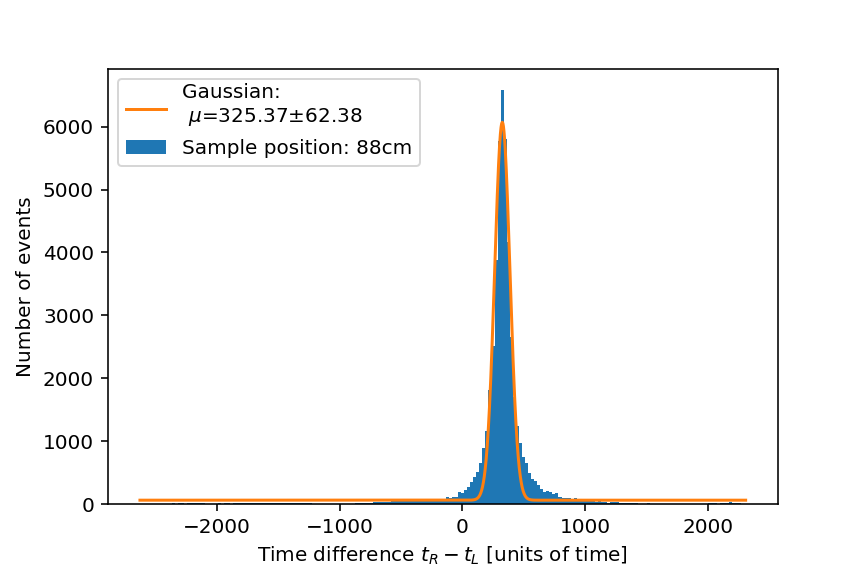
\includegraphics[width=\linewidth]{Plots/Pos/88cm.png}
\end{subfigure}
\begin{subfigure}[c]{0.48\linewidth}
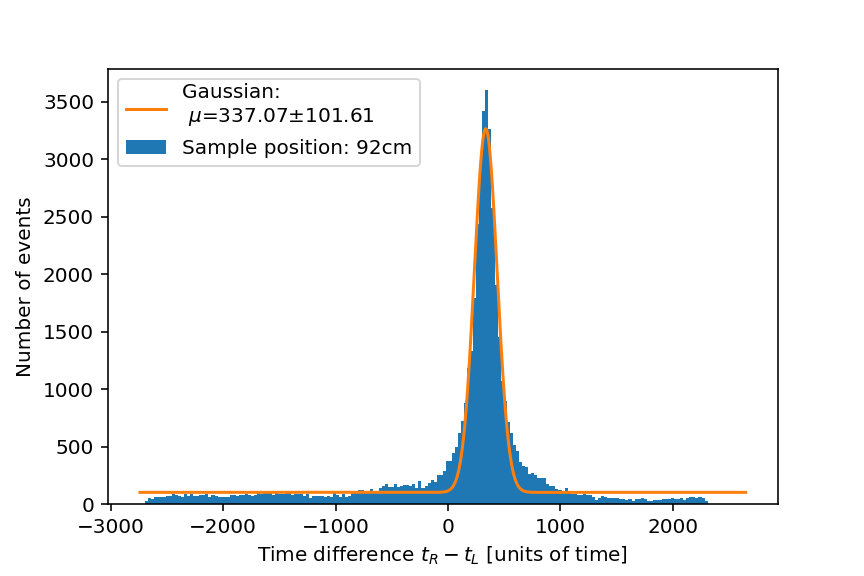
\includegraphics[width=\linewidth]{Plots/Pos/92cm.png}
\end{subfigure}

\medskip
\begin{subfigure}{0.48\textwidth}
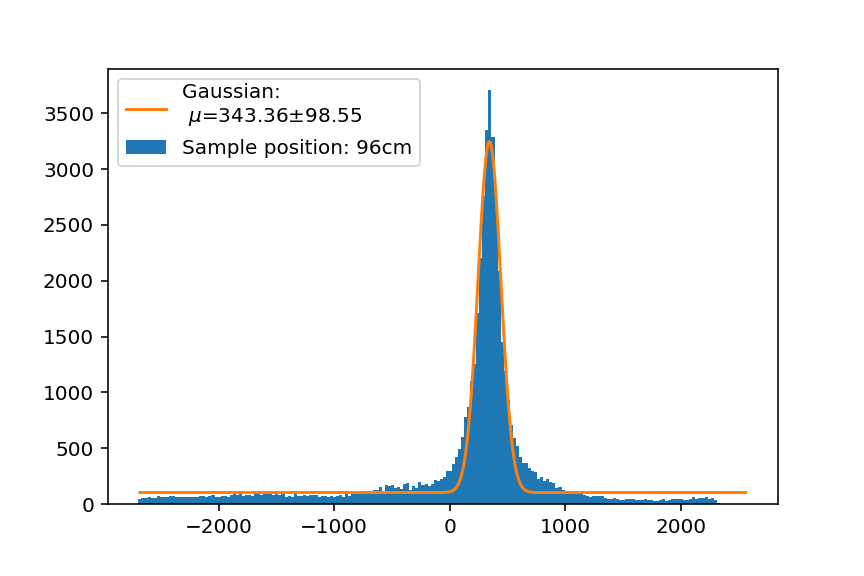
\includegraphics[width=\linewidth]{Plots/Pos/96cm.png}
\end{subfigure}
\begin{subfigure}[c]{0.48\linewidth}
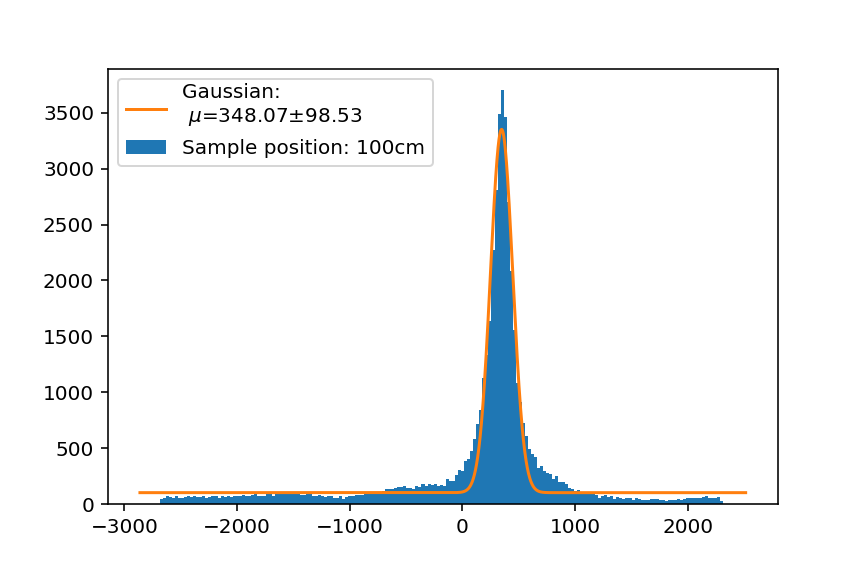
\includegraphics[width=\linewidth]{Plots/Pos/100cm.png}
\end{subfigure}

\medskip
\begin{subfigure}{0.48\textwidth}
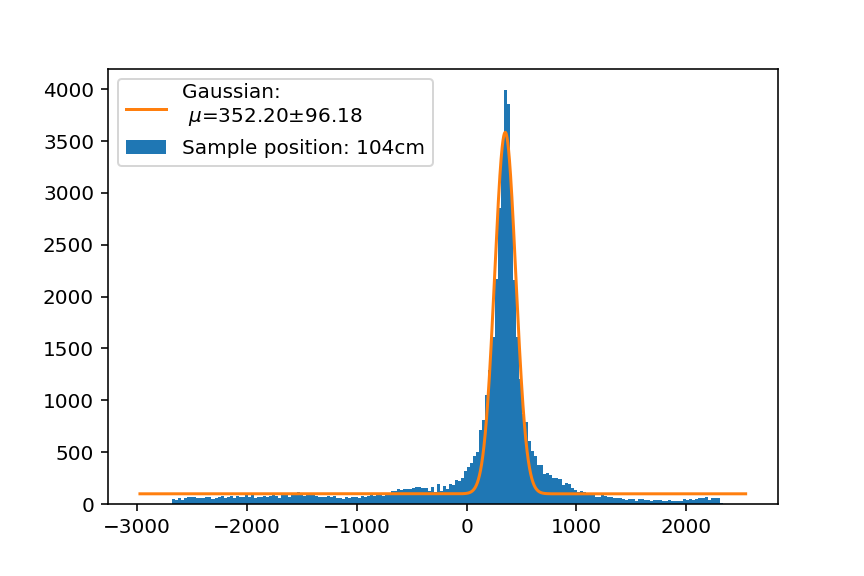
\includegraphics[width=\linewidth]{Plots/Pos/104cm.png}
\end{subfigure}
\begin{subfigure}[c]{0.48\linewidth}
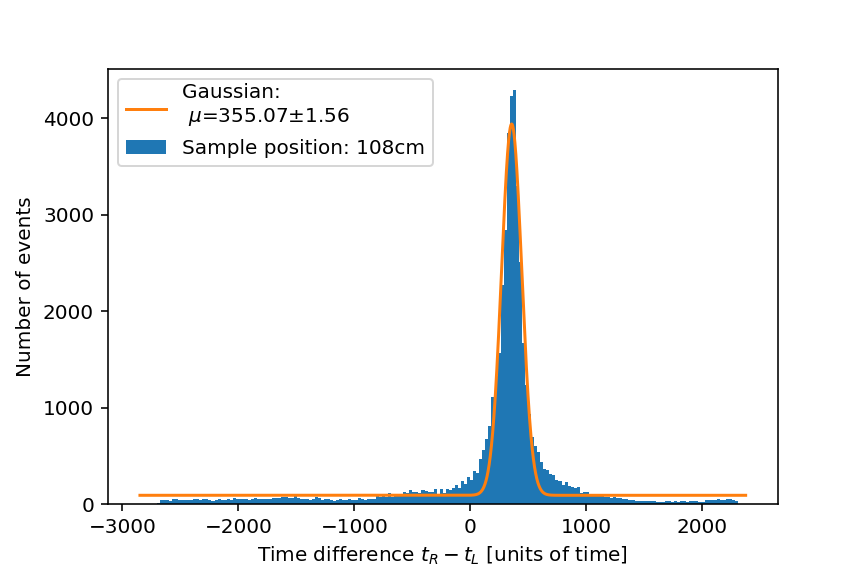
\includegraphics[width=\linewidth]{Plots/Pos/108cm.png}
\end{subfigure}

\medskip
\begin{subfigure}{0.48\textwidth}
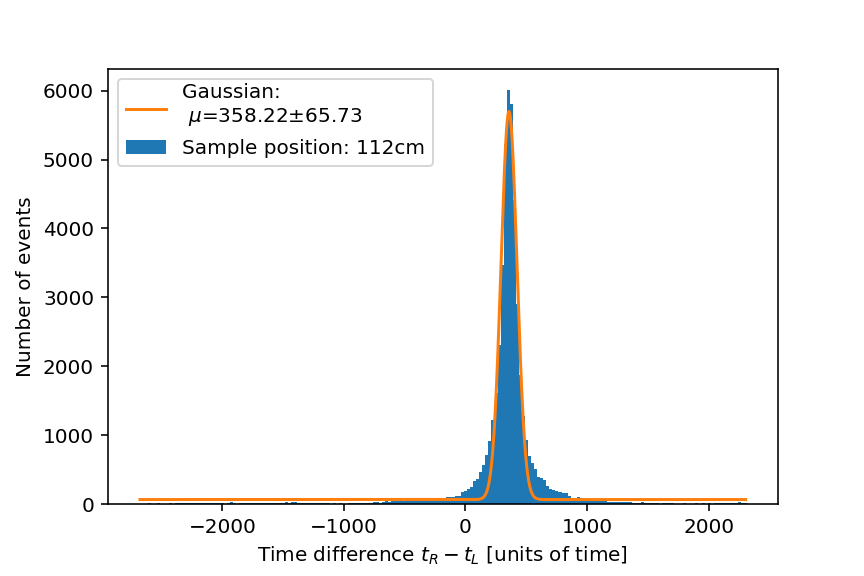
\includegraphics[width=\linewidth]{Plots/Pos/112cm.png}
\end{subfigure}
\begin{subfigure}[c]{0.48\linewidth}
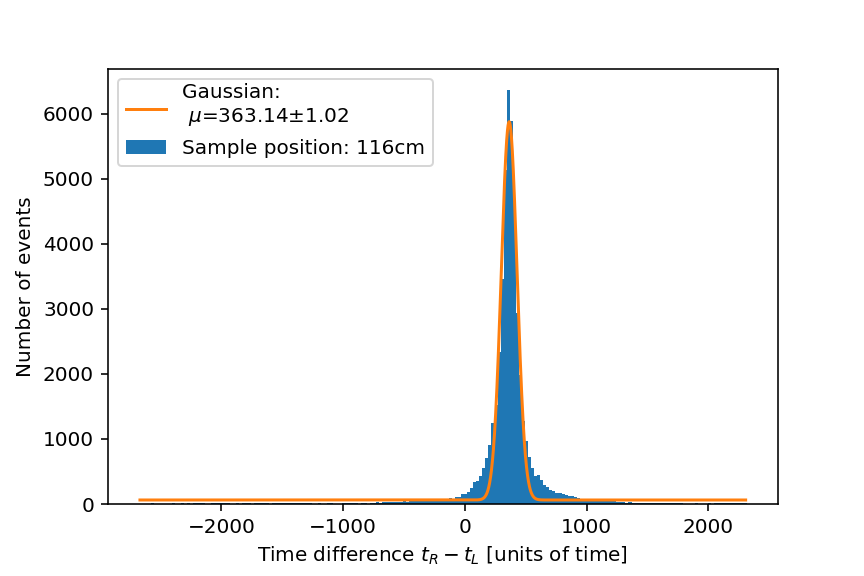
\includegraphics[width=\linewidth]{Plots/Pos/116cm.png}
\end{subfigure}
\caption{Histograms for the c calculation in chapter \ref{c determination}. Part III }
\end{figure}

\begin{figure}[H]
\centering
\medskip
\begin{subfigure}{0.48\textwidth}
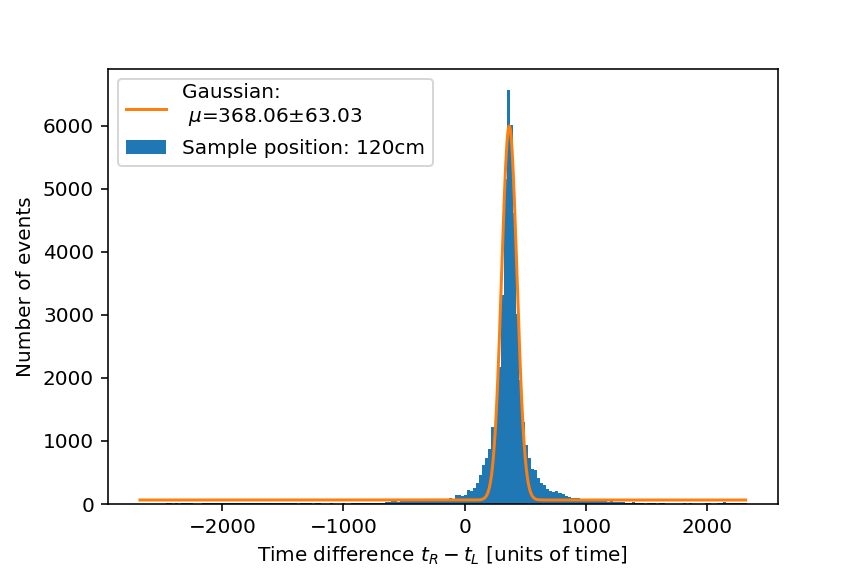
\includegraphics[width=\linewidth]{Plots/Pos/120cm.png}
\end{subfigure}
\begin{subfigure}[c]{0.48\linewidth}
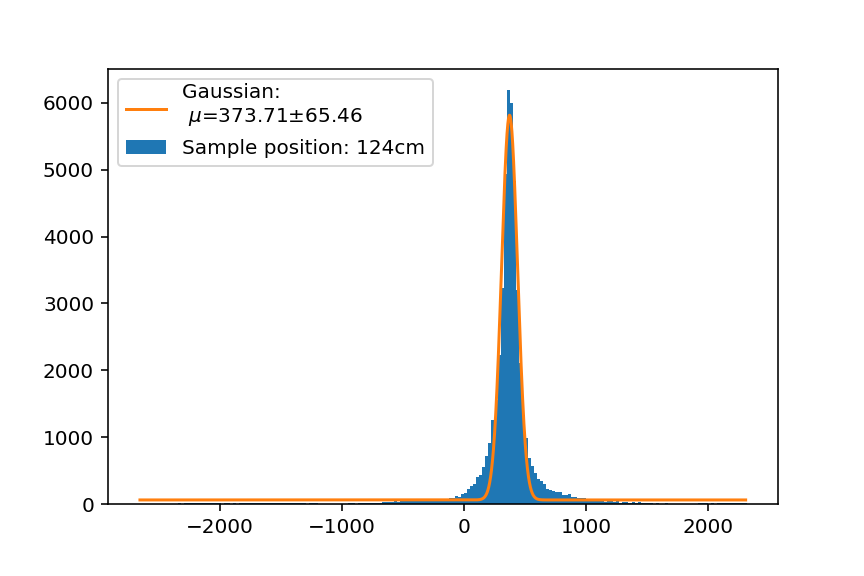
\includegraphics[width=\linewidth]{Plots/Pos/124cm.png}
\end{subfigure}

\medskip
\begin{subfigure}{0.48\textwidth}
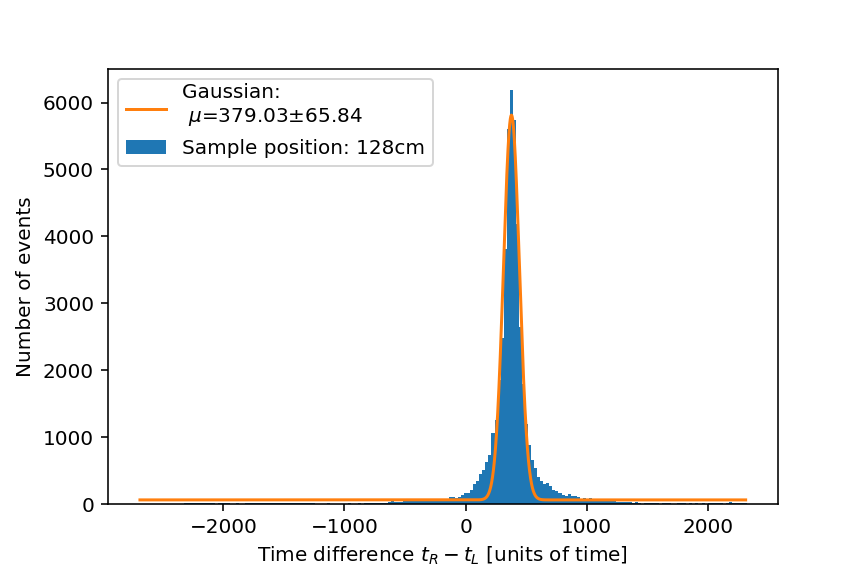
\includegraphics[width=\linewidth]{Plots/Pos/128cm.png}
\end{subfigure}
\begin{subfigure}[c]{0.48\linewidth}
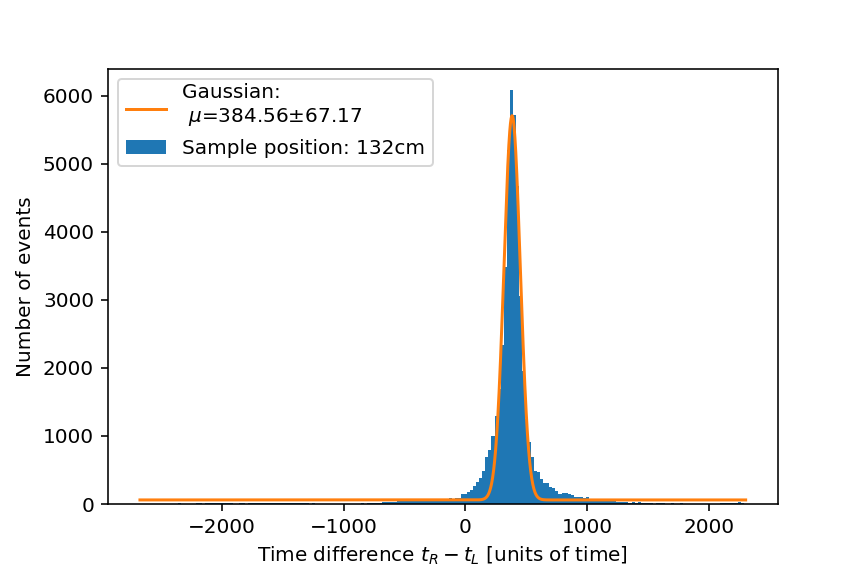
\includegraphics[width=\linewidth]{Plots/Pos/132cm.png}
\end{subfigure}

\medskip
\begin{subfigure}{0.48\textwidth}
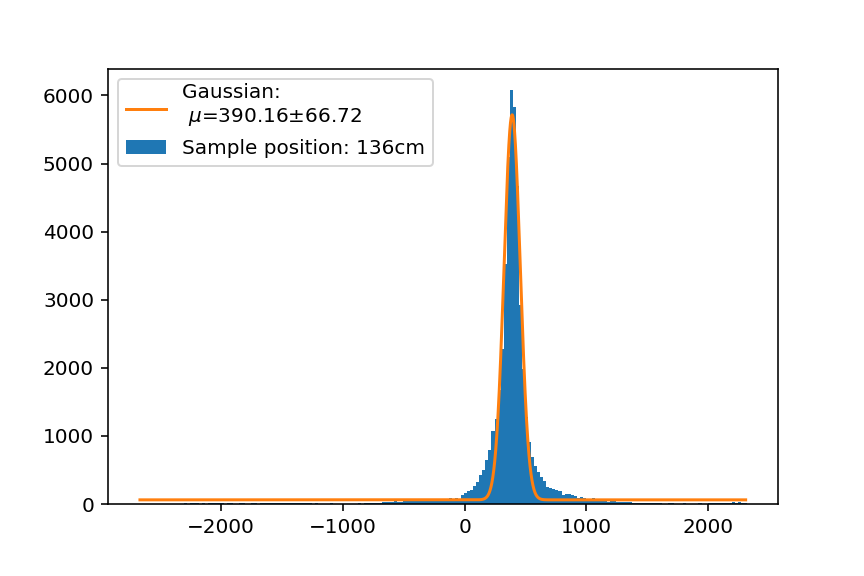
\includegraphics[width=\linewidth]{Plots/Pos/136cm.png}
\end{subfigure}
\begin{subfigure}[c]{0.48\linewidth}
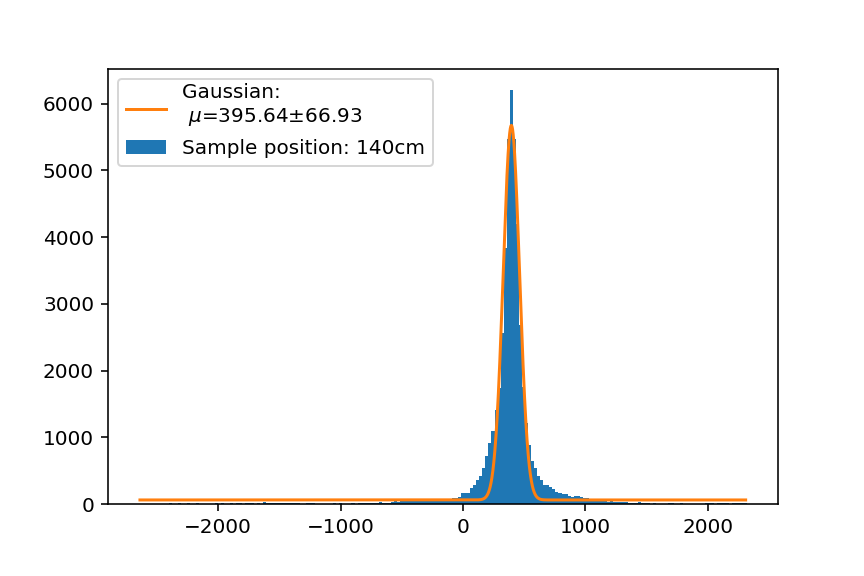
\includegraphics[width=\linewidth]{Plots/Pos/140cm.png}
\end{subfigure}

\medskip
\begin{subfigure}{0.48\textwidth}
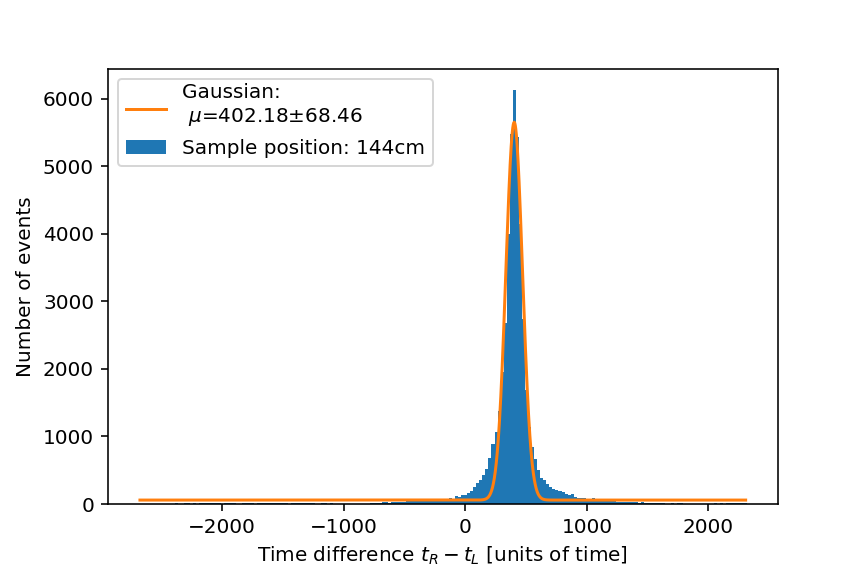
\includegraphics[width=\linewidth]{Plots/Pos/144cm.png}
\end{subfigure}
\begin{subfigure}[c]{0.48\linewidth}
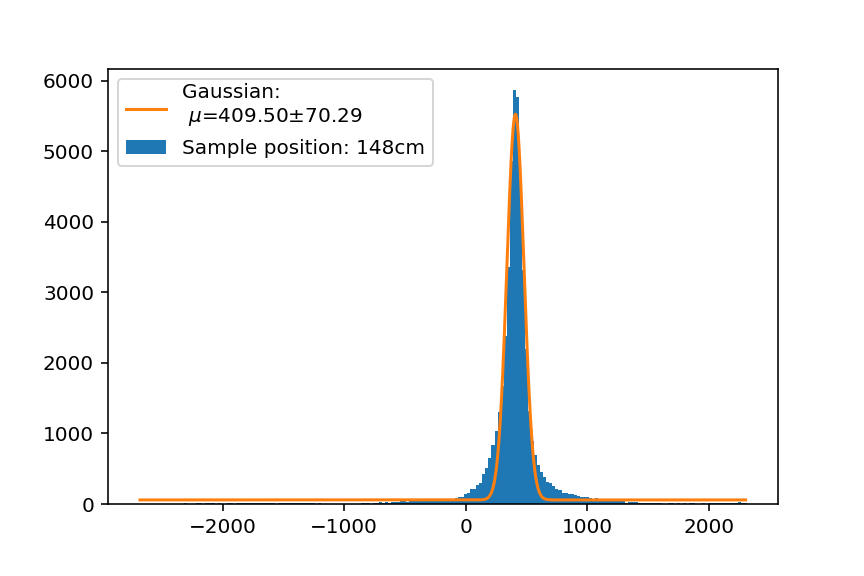
\includegraphics[width=\linewidth]{Plots/Pos/148cm.png}
\end{subfigure}
\caption{Histograms for the time calibration in chapter \ref{time}. Part IV }
\end{figure}

\begin{figure}[H]
\centering
\medskip
\begin{subfigure}{0.48\textwidth}
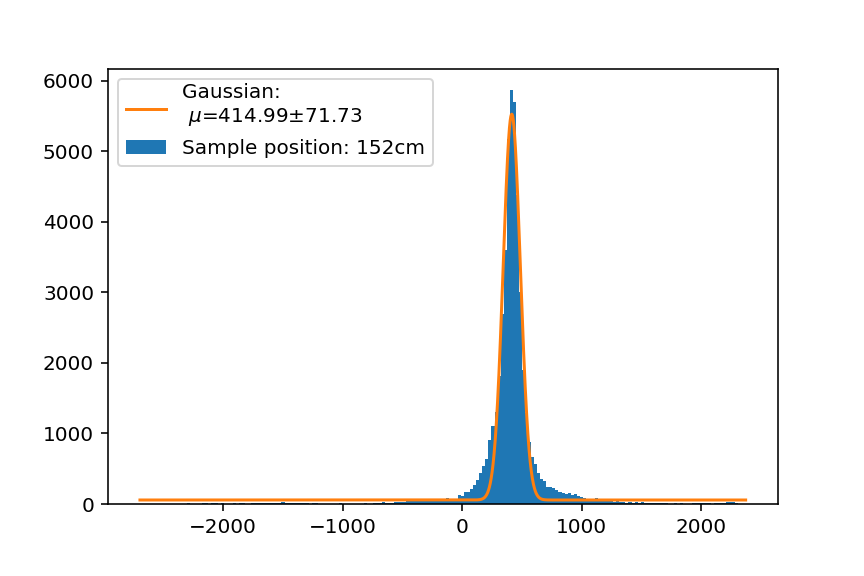
\includegraphics[width=\linewidth]{Plots/Pos/152cm.png}
\end{subfigure}
\begin{subfigure}[c]{0.48\linewidth}
\includegraphics[width=\linewidth]{Plots/Pos/156cm.png}
\end{subfigure}

\medskip
\begin{subfigure}{0.48\textwidth}
\includegraphics[width=\linewidth]{Plots/Pos/160cm.png}
\end{subfigure}
\begin{subfigure}[c]{0.48\linewidth}
\includegraphics[width=\linewidth]{Plots/Pos/164cm.png}
\end{subfigure}

\medskip
\begin{subfigure}{0.48\textwidth}
\includegraphics[width=\linewidth]{Plots/Pos/168cm.png}
\end{subfigure}
\begin{subfigure}[c]{0.48\linewidth}
\includegraphics[width=\linewidth]{Plots/Pos/172cm.png}
\end{subfigure}

\medskip
\begin{subfigure}{0.48\textwidth}
\includegraphics[width=\linewidth]{Plots/Pos/176cm.png}
\end{subfigure}
\begin{subfigure}[c]{0.48\linewidth}
\includegraphics[width=\linewidth]{Plots/Pos/180cm.png}
\end{subfigure}
\caption{Histograms for the c calculation in chapter \ref{c determination}. Part V }
\end{figure}


\newpage
\begin{thebibliography}{}

\bibitem{script} VMEScript.pdf, script for this experiment.

\bibitem{refractive index} \begin{verbatim}
https://eljentechnology.com/images/products/data_sheets/
  EJ-228_EJ-230.pdf
 https://www.crystals.saint-gobain.com/sites/imdf.crystals.com/
  files/documents/sgc-bc400-404-408-412-416-data-sheet.pdf
\end{verbatim} 


\end{thebibliography}
\end{document}

